\RequirePackage{luatex85}
\PassOptionsToPackage{unicode}{hyperref}
\PassOptionsToPackage{naturalnames}{hyperref}
\documentclass{article}
% \documentclass[english,aps,prd,onecolumn,showpacs,superscriptaddress,groupedaddress,fixfloats]{revtex4-1}
\usepackage{geometry}
\usepackage[cm]{fullpage}
\usepackage{parskip}
\usepackage{physics}
\usepackage{amsmath}
\usepackage{amssymb}
\usepackage{xcolor}
\usepackage[colorlinks,linkcolor=blue,citecolor=green]{hyperref}
\usepackage{array}
\usepackage{longtable}
\usepackage{multirow}
\usepackage{comment}
\usepackage{graphicx}
\usepackage{cite}
\usepackage{amsfonts}
\usepackage{bm}
\usepackage{slashed}
\usepackage{dsfont}
\usepackage{mathtools}
\usepackage[compat=1.1.0]{tikz-feynman}
\usepackage{tikz}
\usetikzlibrary{hobby}
\usepackage{pgfplots}
\pgfplotsset{compat=newest}
\usepackage{simpler-wick} 
\usepackage{mathrsfs}
\usepackage{xparse}
\usepackage{enumerate}
\usepackage{extarrows}
\usepackage[caption=false]{subfig}\renewcommand*\thesubfigure{\arabic{subfigure}} 
% ==============================================================================
% Endnotes
% ==============================================================================
\usepackage{enotez}
% HOWTO: 
% \endnote{}
% Print the notes by adding the following to the end of the document: 
% \printendnotes

% ==============================================================================
% Minted
% ==============================================================================
\usepackage{minted}
\usemintedstyle{colorful}

% ==============================================================================
% Changes: comments and highlights
% ==============================================================================
\let\comment\undefined
\usepackage[highlightmarkup=uwave]{changes}

\allowdisplaybreaks

% ==============================================================================
% mathtools
% ==============================================================================
\newcommand\MTkillspecial[1]{% helper macro
	\bgroup
	\catcode`\&=9
	\let\\\relax%
	\scantokens{#1}%
	\egroup
	}
\DeclarePairedDelimiter\BraceM\{\}
\reDeclarePairedDelimiterInnerWrapper\BraceM{star}{
	\mathopen{#1\vphantom{\MTkillspecial{#2}}\kern-\nulldelimiterspace\right.}
	#2
	\mathclose{\left.\kern-\nulldelimiterspace\vphantom{\MTkillspecial{#2}}#3}
	}
\DeclarePairedDelimiter\bracketM{[}{]}
\reDeclarePairedDelimiterInnerWrapper\bracketM{star}{
	\mathopen{#1\vphantom{\MTkillspecial{#2}}\kern-\nulldelimiterspace\right.}
	#2
	\mathclose{\left.\kern-\nulldelimiterspace\vphantom{\MTkillspecial{#2}}#3}
	}
\let\Bqty\relax
\let\bqty\relax
\newcommand{\Bqty}[1]{\BraceM*{#1}}
\newcommand{\bqty}[1]{\bracketM*{#1}}
\DeclarePairedDelimiter\ceil{\lceil}{\rceil}
\DeclarePairedDelimiter\floor{\lfloor}{\rfloor}

% ==============================================================================
% ifthen for User-definition
% ==============================================================================
\usepackage{ifthen}
% HOWTO:
% \ifthenelse{<test>}{<code for true>}{<code for false>}

% ==============================================================================
% User Definition
% ==============================================================================
\newcommand{\red}[1]{{\color{red}#1}}
\newcommand{\mm}[1]{\frac{\dd^4#1}{(2\pi)^4}}
\newcommand{\mme}[1]{\frac{\dd^3\vb{#1}}{(2\pi)^3}}
\newcommand{\mmd}[2][d]{\ifthenelse{\equal{#1}{1}}{\frac{\dd {#2}}{2\pi}}{\frac{\dd^{#1}{#2}}{(2\pi)^{#1}}}}

\newcommand{\glprog}[2]{\int\frac{\dd #1}{2\pi}\frac{ie^{-i#1 #2}}{#1+i\epsilon}}

\makeatletter
\newcommand{\pushright}[1]{\ifmeasuring@#1\else\omit\hfill$\displaystyle#1$\fi\ignorespaces}
\newcommand{\pushleft}[1]{\ifmeasuring@#1\else\omit$\displaystyle#1$\hfill\fi\ignorespaces}
\makeatother

\NewDocumentCommand\NL{s}{%
  \IfBooleanTF#1%
    {\notag\\\times}% If a star is seen
    {\notag\\}%     If no star is seen
}



% ==============================================================================
% Tikz-Feynman Externalization
% ==============================================================================
\usepackage{shellesc}
\usetikzlibrary{external}
\usepgfplotslibrary{external}
\tikzexternalize[shell escape=-enable-write18,prefix=./,system call={lualatex \tikzexternalcheckshellescape -halt-on-error -interaction=batchmode -jobname "\image" "\texsource"},up to date check=md5]

\tikzfeynmanset{
	Eikonal/.style={
		/tikz/draw=none,
		/tikz/decoration={name=none},
		/tikz/postaction={
			/tikz/draw,
			/tikz/double distance=2pt,
			% /tikzfeynman/with arrow=0.5,
		},
	},
	tikzmom/.code n args={4}{
		\def\tempa{#1}
		\def\tempb{#2}
		\def\tempc{#3}
		\def\tempd{#4}

		\ifx \empty\tempa 
			\pgfkeysalso{momentum/arrow shorten={0.15}} % default value
		\else \pgfkeysalso{momentum/arrow shorten={#1}}
		\fi

		\ifx \empty\tempb 
			\pgfkeysalso{momentum/arrow distance={3mm}} % default value
		\else \pgfkeysalso{momentum/arrow distance={#2}}
		\fi

		\ifx \empty\tempc 
			\pgfkeysalso{momentum/label distance={0pt}} % default value
		\else \pgfkeysalso{momentum/label distance={#3}}
		\fi

		\pgfkeysalso{momentum={#4}}
	},
	tikzmom'/.code n args={4}{
		\def\tempa{#1}
		\def\tempb{#2}
		\def\tempc{#3}
		\def\tempd{#4}

		\ifx \empty\tempa 
			\pgfkeysalso{momentum/arrow shorten={0.15}} % default value
		\else \pgfkeysalso{momentum/arrow shorten={#1}}
		\fi

		\ifx \empty\tempb 
			\pgfkeysalso{momentum/arrow distance={3mm}} % default value
		\else \pgfkeysalso{momentum/arrow distance={#2}}
		\fi

		\ifx \empty\tempc 
			\pgfkeysalso{momentum/label distance={0pt}} % default value
		\else \pgfkeysalso{momentum/label distance={#3}}
		\fi

		\pgfkeysalso{momentum'={#4}}
	},
	half right/.append style={
		/tikz/looseness=2
	},
	half left/.append style={
		/tikz/looseness=2
	}
}

% ==============================================================================
% Tikz-Feynman Auxiliary
% ==============================================================================
\def\FDWidth{3cm}
\def\FDHeight{3cm}
\def\FDWidthS{2cm}
\def\FDHeightS{2cm}

\title{Two Loop Matching for Quasi PDF}
\author{Yingsheng Huang}
\begin{document}
\maketitle

\section{Renormalization}
\subsection{One loop diagrams}
\begin{figure}[!htpb]
	\centering\hfil
	\subfloat[]{
		\centering
		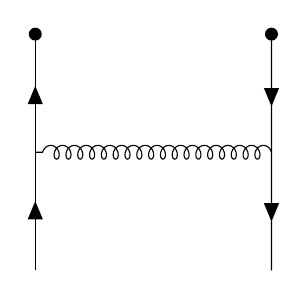
\begin{tikzpicture}[baseline=($(a)!0.5!(exa)$.base)]
			\begin{feynman}
				\node[dot] (a);
				\node[right=\FDWidth of a,dot] (b);
				\vertex[below=\FDHeight of a] (exa);
				\vertex[below=\FDHeight of b] (exb);
				\vertex at ($(exa)!0.5!(a)$) (a1);
				\vertex at ($(exb)!0.5!(b)$) (b1);
				\diagram*{
				% (a) --[Eikonal] (b);
				(exa) --[fermion] (a1) --[fermion] (a);
				(b) --[fermion] (b1) --[fermion] (exb);
				(b1) --[gluon] (a1);
				};
			\end{feynman}
		\end{tikzpicture}
		\label{2:nogl}
	}\hfil
	\subfloat[]{
		\centering
		\null\hfill%
		\begin{tikzpicture}[baseline=($(a)!0.5!(exa)$.base)]
			\begin{feynman}
				\node[dot] (a);
				\node[right=\FDWidth of a,dot] (b);
				\vertex at ($(a)!0.5!(b)$) (o);
				\vertex[below=\FDHeight of a] (exa);
				\vertex[below=\FDHeight of b] (exb);
				\vertex at ($(exa)!0.5!(a)$) (a1);
				\vertex at ($(exb)!0.5!(b)$) (b1);
				\diagram*{
				(o) --[Eikonal] (b);
				(exa) --[fermion] (a1) --[fermion] (a);
				(b) --[fermion] (exb);
				(a1) --[gluon] (o);
				};
			\end{feynman}
		\end{tikzpicture}\hfill+\hfill
		\begin{tikzpicture}[baseline=($(a)!0.5!(exa)$.base)]
			\begin{feynman}
				\node[dot] (a);
				\node[right=\FDWidth of a,dot] (b);
				\vertex at ($(a)!0.5!(b)$) (o);
				\vertex[below=\FDHeight of a] (exa);
				\vertex[below=\FDHeight of b] (exb);
				\vertex at ($(exa)!0.5!(a)$) (a1);
				\vertex at ($(exb)!0.5!(b)$) (b1);
				\diagram*{
				(a) --[Eikonal] (o);
				(exa) --[fermion] (a);
				(b) --[fermion] (b1) --[fermion] (exb);
				(b1) --[gluon] (o);
				};
			\end{feynman}
		\end{tikzpicture}\hfill\null%
		\label{2-`}
	}\hfil
	\subfloat[]{
		\centering
		\begin{tikzpicture}[baseline=($(a)!0.5!(exa)$.base)]
			\begin{feynman}
				\node[dot] (a);
				\node[right=\FDWidth of a,dot] (b);
				\vertex at ($(a)!0.3!(b)$) (o1);
				\vertex at ($(a)!0.7!(b)$) (o2);
				\vertex[below=\FDHeight of a] (exa);
				\vertex[below=\FDHeight of b] (exb);
				\diagram*{
				(a) --[Eikonal] (o1);
				(b) --[Eikonal] (o2);
				(exa) --[fermion] (a);
				(b) --[fermion] (exb);
				(o1) --[gluon, half right] (o2);
				};
			\end{feynman}
		\end{tikzpicture}
		\label{2-v-}
	}\hfil\\\hfil
	\subfloat[]{
		\centering
		\null\hfill
		\begin{tikzpicture}[baseline=($(a)!0.5!(exa)$.base)]
			\begin{feynman}
				\node[dot] (a);
				\node[right=\FDWidth of a,dot] (b);
				\vertex at ($(a)!0.5!(b)$) (o);
				\vertex[below=\FDHeight of a] (exa);
				\vertex[below=\FDHeight of b] (exb);
				\vertex at ($(exa)!0.5!(a)$) (a1);
				\vertex at ($(exb)!0.5!(b)$) (b1);
				\diagram*{
				(o) --[Eikonal] (a);
				(exa) --[fermion] (a1) --[fermion] (a);
				(b) --[fermion] (exb);
				(a1) --[gluon] (o);
				};
			\end{feynman}
		\end{tikzpicture}\hfill+\hfill
		\begin{tikzpicture}[baseline=($(a)!0.5!(exa)$.base)]
			\begin{feynman}
				\node[dot] (a);
				\node[right=\FDWidth of a,dot] (b);
				\vertex at ($(a)!0.5!(b)$) (o);
				\vertex[below=\FDHeight of a] (exa);
				\vertex[below=\FDHeight of b] (exb);
				\vertex at ($(exa)!0.5!(a)$) (a1);
				\vertex at ($(exb)!0.5!(b)$) (b1);
				\diagram*{
				(b) --[Eikonal] (o);
				(exa) --[fermion] (a);
				(b) --[fermion] (b1) --[fermion] (exb);
				(b1) --[gluon] (o);
				};
			\end{feynman}
		\end{tikzpicture}\hfill\null
		\label{2`-}
	}\hfil
	\subfloat[]{
		\centering
		\null\hfill
		\begin{tikzpicture}[baseline=($(a)!0.5!(exa)$.base)]
			\begin{feynman}
				\node[dot] (a);
				\node[right=\FDWidth of a,dot] (b);
				\vertex at ($(a)!0.5!(b)$) (o);
				\vertex at ($(a)!0.2!(b)$) (o1);
				\vertex at ($(a)!0.8!(b)$) (o2);
				\vertex[below=\FDHeight of a] (exa);
				\vertex[below=\FDHeight of b] (exb);
				\diagram*{
				(a) --[Eikonal] (o);
				(exa) --[fermion] (a);
				(b) --[fermion] (exb);
				(o1) --[gluon, half right] (o);
				};
			\end{feynman}
		\end{tikzpicture}\hfill+\hfill
		\begin{tikzpicture}[baseline=($(a)!0.5!(exa)$.base)]
			\begin{feynman}
				\node[dot] (a);
				\node[right=\FDWidth of a,dot] (b);
				\vertex at ($(a)!0.5!(b)$) (o);
				\vertex at ($(a)!0.2!(b)$) (o1);
				\vertex at ($(a)!0.8!(b)$) (o2);
				\vertex[below=\FDHeight of a] (exa);
				\vertex[below=\FDHeight of b] (exb);
				\diagram*{
				(b) --[Eikonal] (o);
				(exa) --[fermion] (a);
				(b) --[fermion] (exb);
				(o) --[gluon, half right] (o2);
				};
			\end{feynman}
		\end{tikzpicture}
		\label{2o-}
	}\hfil\\\hfil
	\subfloat[]{
		\centering
		\null\hfill
		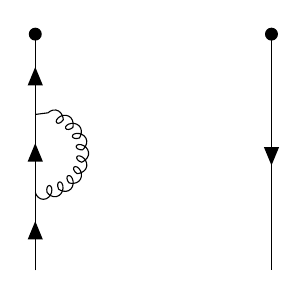
\begin{tikzpicture}[baseline=($(a)!0.5!(exa)$.base)]
			\begin{feynman}
				\node[dot] (a);
				\node[right=\FDWidth of a,dot] (b);
				\vertex[below=\FDHeight of a] (exa);
				\vertex[below=\FDHeight of b] (exb);
				\vertex at ($(exa)!0.33!(a)$) (a1);
				\vertex at ($(exa)!0.66!(a)$) (a2);
				\diagram*{
				% (a) --[Eikonal] (b);
				(exa) --[fermion] (a1) --[fermion] (a2) --[fermion] (a);
				(b) --[fermion] (exb);
				(a1) --[gluon, half right,looseness=2] (a2);
				};
			\end{feynman}
		\end{tikzpicture}\hfil+\hfil
		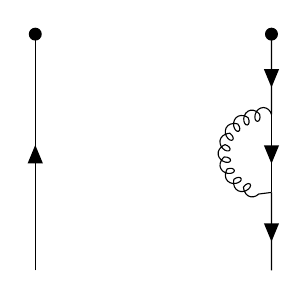
\begin{tikzpicture}[baseline=($(a)!0.5!(exa)$.base)]
			\begin{feynman}
				\node[dot] (a);
				\node[right=\FDWidth of a,dot] (b);
				\vertex[below=\FDHeight of a] (exa);
				\vertex[below=\FDHeight of b] (exb);
				\vertex at ($(exb)!0.33!(b)$) (b1);
				\vertex at ($(exb)!0.66!(b)$) (b2);
				\diagram*{
				% (a) --[Eikonal] (b);
				(exa) --[fermion] (a);
				(b) --[fermion] (b2) --[fermion] (b1) --[fermion] (exb);
				(b2) --[gluon, half right,looseness=2] (b1);
				};
			\end{feynman}
		\end{tikzpicture}\hfill\null
	}\hfil
	\caption{Diagrams of quasi PDF in Feynman gauge. }
\end{figure}
\subsection{Vertex corrections}
According to \cite{Ji:2015jwa}, the vertex correction diagrams in axial gauge (which corresponds to varieties of diagrams in general covariant gauge) don't have total UV divergence. Rather, they only have subdivergence for sub-diagrams. For example the first column (which involves Figure~3), second row of Table~1 in \cite{Ji:2015jwa} is composed of $\tilde q_{11}$ and $\tilde q_{12}$, thus we can find some representative diagrams and extract those components ($l\equiv l_1+l_2, \Delta l\equiv l_1-l_2$)
\begin{align}
	&\begin{tikzpicture}[transform shape,scale=1,baseline=($(a)!0.5!(exa)$.base)]
		\begin{feynman}
			\node[dot] (a);
			\node[right=\FDWidth of a,dot] (b);
			\vertex at ($(a)!0.66!(b)$) (o);
			\vertex[below=\FDHeight of a] (exa);
			\vertex[below=\FDHeight of b] (exb);
			\vertex at ($(exa)!0.3!(a)$) (a1);
			\vertex at ($(exa)!0.7!(a)$) (a2);
			\vertex at ($(a1)!0.5!(a2)!1.2!-90:(a2)$) (g1);
			\vertex at ($(exb)!0.5!(b)$) (b1);
			\diagram*{
			(o) --[Eikonal,momentum=\(P-l_2\)] (b);
			(exa) --[fermion,momentum=\(P\)] (a1) --[fermion,momentum=\(l_1\)] (a2) --[fermion,momentum=\(l_2\)] (a);
			(a1) --[gluon,half right,looseness=2] (a2);
			(a1) --[quarter right,tikzmom'={0.2}{2mm}{-2pt}{$P-l_1$},draw=none] (g1) --[quarter right,tikzmom'={0.2}{2mm}{-2pt}{$\Delta l$},draw=none] (a2);
			(b) --[fermion,momentum=\(P\)] (exb);
			(g1) --[gluon,tikzmom'={0.2}{2mm}{-2pt}{$P-l_2$}] (o);
			};
		\end{feynman}
	\end{tikzpicture}\propto \int\mmd[d]{l_1}\mmd[d]{l_2}\frac{1}{\bqty{\slashed l_1-m}\bqty{\slashed l_2-m}\bqty{(P-l_1)^2}\bqty{(l_1-l_2)^2}\bqty{(P-l_2)^2}\bqty{n\cdot(P-l_2)}}
\end{align}
Take the $l_1\gg l_2$ limit, the integrand becomes
\begin{align}
	\frac{1}{\bqty{\slashed l_1-m}\bqty{(P-l_1)^2}\bqty{l_1^2}\bqty{\slashed l_2-m}\bqty{(P-l_2)^2}\bqty{n\cdot(P-l_2)}}
\end{align}
The integral involving $l_2$ is exactly the integral of $\tilde q_{12}$. By adding the gluon self-interacting vertex we can see that the sub-diagram is logarithmic divergent. 

Take the $l_2\gg l_1$ limit, the integrand becomes
\begin{align}
	\frac{1}{\bqty{\slashed l_1-m}\bqty{(P-l_1)^2}\bqty{l_2^2}\bqty{\slashed l_2-m}\bqty{(P-l_2)^2}\bqty{n\cdot(P-l_2)}}
\end{align}

There's another limit where hard loop momentum flows through all paths except the one that's $\Delta l$ in our current diagram. This configuration gives a finite integral and a power-divergent integral which happens to be a scaleless integral as well. Thus this configuration won't contribute. 

What we extracted above is only the $\tilde q_{12}$ part, now we will try on the $\tilde q_{11}$ part
\begin{align}
	&\begin{tikzpicture}[transform shape,scale=1,baseline=($(a)!0.5!(exa)$.base)]
		\begin{feynman}
			\node[dot] (a);
			\node[right=\FDWidth of a,dot] (b);
			\vertex at ($(a)!0.66!(b)$) (o);
			\vertex[below=\FDHeight of a] (exa);
			\vertex[below=\FDHeight of b] (exb);
			\vertex at ($(exa)!0.25!(a)$) (a1);
			\vertex at ($(exa)!0.75!(a)$) (a2);
			\vertex at ($(exa)!0.5!(a)$) (am);
			\vertex at ($(exb)!0.5!(b)$) (bm);
			\diagram*{
			(exa) --[fermion,momentum=\(P\)] (a1) --[fermion,tikzmom'={0.3}{2mm}{-1pt}{$l_1$}] (am) --[fermion,tikzmom'={0.3}{2mm}{-1pt}{$l_1+l_2$}] (a2) --[fermion,momentum=\(P+l_2\)] (a);
			(a1) --[gluon,half left,looseness=2,tikzmom={0.3}{}{}{$P-l_1$}] (a2);
			(b) --[fermion,momentum=\(P+l_2\)] (bm)--[fermion,momentum=\(P\)] (exb);
			(bm) --[gluon,tikzmom={0.3}{}{}{$l_2$}] (am);
			};
		\end{feynman}
	\end{tikzpicture}\notag\\
	&\propto \int\mmd[d]{l_1}\mmd[d]{l_2}\frac{1}{\bqty{\slashed l_1-m}\bqty{\slashed l_1+\slashed l_2-m}\bqty{\slashed P+\slashed l_2-m}\bqty{\slashed P+\slashed l_2-m}\bqty{(P-l_1)^2}\bqty{l_2^2}}
\end{align}
In the $l_1\gg l_2$ limit we have 
\begin{align}
	\frac{1}{\bqty{\slashed l_1-m}\bqty{\slashed l_1-m}\bqty{(P-l_1)^2}\bqty{\slashed P+\slashed l_2-m}\bqty{\slashed P+\slashed l_2-m}\bqty{l_2^2}}
\end{align}
and $\tilde q_{11}$ is factorized out. 

Another example is the sixth row
\begin{align}
	\begin{tikzpicture}[transform shape,scale=1,baseline=($(a)!0.5!(exa)$.base)]
		\begin{feynman}
			\node[dot] (a);
			\node[right=\FDWidth of a,dot] (b);
			\vertex at ($(a)!0.5!(b)$) (o);
			\vertex at ($(a)!0.3!(b)$) (o1);
			\vertex at ($(a)!0.8!(b)$) (o2);
			\vertex[below=\FDHeight of a] (exa);
			\vertex[below=\FDHeight of b] (exb);
			\vertex at ($(exa)!0.4!(a)$) (a1);
			\diagram*{
			(o1) --[Eikonal] (o) --[Eikonal,tikzmom={0.2}{2mm}{-2pt}{$l_2$}] (o2) --[Eikonal] (b);
			(exa) --[fermion,momentum=\(P\)] (a1) --[fermion,momentum=\(l_1\)] (a);
			(b) --[fermion,momentum=\(P\)] (exb);
			(o) --[gluon, half right,tikzmom'={0.2}{2mm}{-2pt}{$P-l_1-l_2$}] (o2);
			(a1) --[gluon,tikzmom'={0.2}{2mm}{-2pt}{$P-l_1$}] (o1);
			};
		\end{feynman}
	\end{tikzpicture}\propto
	\int\mmd[d]{l_1}\mmd[d]{l_2}\frac{1}{\bqty{\slashed l_1-m}\bqty{(P-l_1)^2}\bqty{(P-l_1-l_2)^2}\bqty{n\cdot(P-l_1)}\bqty{n\cdot l_2}\bqty{n\cdot(P-l_1)}}
\end{align}
Take the $l_2\gg l_1$ limit, the integrand becomes
\begin{align}
	\frac{1}{\bqty{\slashed l_1-m}\bqty{(P-l_1)^2}\bqty{n\cdot(P-l_1)}\bqty{n\cdot(P-l_1)}\bqty{n\cdot l_2}\bqty{(P-l_2)^2}}
\end{align}
and the integral involving $l_2$ should give something proportional to $n\cot (P-l_1)$, thus cancels one eikonal propagator, the remainder is the integral of $\tilde q_{12}$. 

\section{Real Diagrams}
\subsection{All diagrams}
Figure~\ref{re:sc} lists all self-conjugated real diagrams, and Figure~\ref{re:c} lists all non-self-conjugated diagrams, excluding their conjugates. 
\renewcommand*\thesubfigure{\roman{subfigure}} 
\begin{figure}[!hbtp]
	\centering\null\hfil
	\subfloat[10]{
		\begin{tikzpicture}[transform shape,scale=1,baseline=($(a)!0.5!(exa)$.base)]
			\begin{feynman}
				\node[dot] (a);
				\node[right=\FDWidth of a,dot] (b);
				\vertex[below=\FDHeight of a] (exa);
				\vertex[below=\FDHeight of b] (exb);
				% 
				\vertex at ($(a)!0.33!(b)$) (o13);
				\vertex at ($(a)!0.66!(b)$) (o23);
				\vertex at ($(a)!0.25!(b)$) (o14);
				\vertex at ($(a)!0.5!(b)$) (o12);
				\vertex at ($(a)!0.75!(b)$) (o34);
				% 
				\vertex at ($(a)!0.2!(b)$) (o15);
				\vertex at ($(a)!0.4!(b)$) (o25);
				\vertex at ($(a)!0.6!(b)$) (o35);
				\vertex at ($(a)!0.8!(b)$) (o45);
				% 
				\vertex at ($(o13)+1/4*(0,-\FDHeight)$) (o13m);
				\vertex at ($(o23)+1/4*(0,-\FDHeight)$) (o23m);
				% 
				\vertex at ($(exa)!0.25!(a)$) (a14);
				\vertex at ($(exa)!0.5!(a)$) (a12);
				\vertex at ($(exa)!0.75!(a)$) (a34);
				\vertex at ($(exa)!0.33!(a)$) (a13);
				\vertex at ($(exa)!0.66!(a)$) (a23);
				% 
				\vertex at ($(exb)!0.25!(b)$) (b14);
				\vertex at ($(exb)!0.5!(b)$) (b12);
				\vertex at ($(exb)!0.75!(b)$) (b34);
				\vertex at ($(exb)!0.33!(b)$) (b13);
				\vertex at ($(exb)!0.66!(b)$) (b23);
				% 
				\vertex at ($(a12)!0.33!(b12)$) (ab13);
				\vertex at ($(a12)!0.66!(b12)$) (ab23);
				\vertex at ($(a12)!0.5!(b12)$) (ab12);
				% 
				\vertex at ($(a14)!0.5!(a34)!1.2!-90:(a34)$) (g1);
				% 
				\diagram*{
					(a) --[Eikonal] (o13);
					(o23) --[Eikonal] (b);
					(exa) --[fermion] (a);
					(b) --[fermion] (exb);
					(o13) --[gluon] (o13m);
					(o23) --[gluon] (o23m);
					(o13m) --[gluon,half right,looseness=1.5] (o23m);
					(o13m) --[gluon] (o23m);
				};
			\end{feynman}
		\end{tikzpicture}
		\label{}
	}\hfil
	\subfloat[11]{
		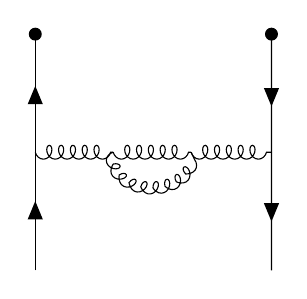
\begin{tikzpicture}[transform shape,scale=1,baseline=($(a)!0.5!(exa)$.base)]
			\begin{feynman}
				\node[dot] (a);
				\node[right=\FDWidth of a,dot] (b);
				\vertex[below=\FDHeight of a] (exa);
				\vertex[below=\FDHeight of b] (exb);
				% 
				\vertex at ($(a)!0.33!(b)$) (o13);
				\vertex at ($(a)!0.66!(b)$) (o23);
				\vertex at ($(a)!0.25!(b)$) (o14);
				\vertex at ($(a)!0.5!(b)$) (o12);
				\vertex at ($(a)!0.75!(b)$) (o34);
				% 
				\vertex at ($(a)!0.2!(b)$) (o15);
				\vertex at ($(a)!0.4!(b)$) (o25);
				\vertex at ($(a)!0.6!(b)$) (o35);
				\vertex at ($(a)!0.8!(b)$) (o45);
				% HOWTO: One can modify this to get vertexes lower than the gauge link line. 
				\vertex at ($(o13)+1/4*(0,-\FDHeight)$) (o13m);
				\vertex at ($(o23)+1/4*(0,-\FDHeight)$) (o23m);
				% 
				\vertex at ($(exa)!0.25!(a)$) (a14);
				\vertex at ($(exa)!0.5!(a)$) (a12);
				\vertex at ($(exa)!0.75!(a)$) (a34);
				\vertex at ($(exa)!0.33!(a)$) (a13);
				\vertex at ($(exa)!0.66!(a)$) (a23);
				% 
				\vertex at ($(exb)!0.25!(b)$) (b14);
				\vertex at ($(exb)!0.5!(b)$) (b12);
				\vertex at ($(exb)!0.75!(b)$) (b34);
				\vertex at ($(exb)!0.33!(b)$) (b13);
				\vertex at ($(exb)!0.66!(b)$) (b23);
				% 
				\vertex at ($(a12)!0.33!(b12)$) (ab13);
				\vertex at ($(a12)!0.66!(b12)$) (ab23);
				\vertex at ($(a12)!0.5!(b12)$) (ab12);
				% 
				\vertex at ($(a14)!0.5!(a34)!1.2!-90:(a34)$) (g1);
				% 
				\diagram*{
					(exa) --[fermion] (a12) --[fermion] (a);
					(b) --[fermion] (b12) --[fermion] (exb);
					(a12) --[gluon] (ab13) --[gluon] (ab23) --[gluon] (b12);
					(ab13) --[gluon,half right] (ab23);
				};
			\end{feynman}
		\end{tikzpicture}
		\label{}
	}\hfil
	\subfloat[26]{
		\begin{tikzpicture}[transform shape,scale=1,baseline=($(a)!0.5!(exa)$.base)]
			\begin{feynman}
				\node[dot] (a);
				\node[right=\FDWidth of a,dot] (b);
				\vertex[below=\FDHeight of a] (exa);
				\vertex[below=\FDHeight of b] (exb);
				% 
				\vertex at ($(a)!0.33!(b)$) (o13);
				\vertex at ($(a)!0.66!(b)$) (o23);
				\vertex at ($(a)!0.25!(b)$) (o14);
				\vertex at ($(a)!0.5!(b)$) (o12);
				\vertex at ($(a)!0.75!(b)$) (o34);
				% 
				\vertex at ($(a)!0.2!(b)$) (o15);
				\vertex at ($(a)!0.4!(b)$) (o25);
				\vertex at ($(a)!0.6!(b)$) (o35);
				\vertex at ($(a)!0.8!(b)$) (o45);
				% 
				\vertex at ($(o13)+1/4*(0,-\FDHeight)$) (o13m);
				\vertex at ($(o23)+1/4*(0,-\FDHeight)$) (o23m);
				% 
				\vertex at ($(exa)!0.25!(a)$) (a14);
				\vertex at ($(exa)!0.5!(a)$) (a12);
				\vertex at ($(exa)!0.75!(a)$) (a34);
				\vertex at ($(exa)!0.33!(a)$) (a13);
				\vertex at ($(exa)!0.66!(a)$) (a23);
				% 
				\vertex at ($(exb)!0.25!(b)$) (b14);
				\vertex at ($(exb)!0.5!(b)$) (b12);
				\vertex at ($(exb)!0.75!(b)$) (b34);
				\vertex at ($(exb)!0.33!(b)$) (b13);
				\vertex at ($(exb)!0.66!(b)$) (b23);
				% 
				\vertex at ($(a12)!0.33!(b12)$) (ab13);
				\vertex at ($(a12)!0.66!(b12)$) (ab23);
				\vertex at ($(a12)!0.5!(b12)$) (ab12);
				% 
				\vertex at ($(a14)!0.5!(a34)!1.2!-90:(a34)$) (g1);
				% 
				\diagram*{
					(a) --[Eikonal] (o13);
					(o23) --[Eikonal] (b);
					(exa) --[fermion] (a);
					(b) --[fermion] (exb);
					(o13) --[gluon] (o13m);
					(o23) --[gluon] (o23m);
					(o13m) --[ghost,half right,looseness=1.5] (o23m);
					(o13m) --[ghost] (o23m);
				};
			\end{feynman}
		\end{tikzpicture}
		\label{}
	}\hfil
	\subfloat[27]{
		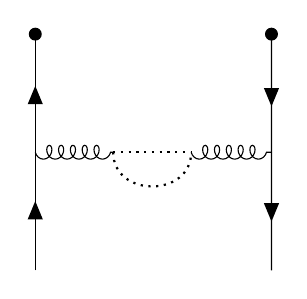
\begin{tikzpicture}[transform shape,scale=1,baseline=($(a)!0.5!(exa)$.base)]
			\begin{feynman}
				\node[dot] (a);
				\node[right=\FDWidth of a,dot] (b);
				\vertex[below=\FDHeight of a] (exa);
				\vertex[below=\FDHeight of b] (exb);
				% 
				\vertex at ($(a)!0.33!(b)$) (o13);
				\vertex at ($(a)!0.66!(b)$) (o23);
				\vertex at ($(a)!0.25!(b)$) (o14);
				\vertex at ($(a)!0.5!(b)$) (o12);
				\vertex at ($(a)!0.75!(b)$) (o34);
				% 
				\vertex at ($(a)!0.2!(b)$) (o15);
				\vertex at ($(a)!0.4!(b)$) (o25);
				\vertex at ($(a)!0.6!(b)$) (o35);
				\vertex at ($(a)!0.8!(b)$) (o45);
				% HOWTO: One can modify this to get vertexes lower than the gauge link line. 
				\vertex at ($(o13)+1/4*(0,-\FDHeight)$) (o13m);
				\vertex at ($(o23)+1/4*(0,-\FDHeight)$) (o23m);
				% 
				\vertex at ($(exa)!0.25!(a)$) (a14);
				\vertex at ($(exa)!0.5!(a)$) (a12);
				\vertex at ($(exa)!0.75!(a)$) (a34);
				\vertex at ($(exa)!0.33!(a)$) (a13);
				\vertex at ($(exa)!0.66!(a)$) (a23);
				% 
				\vertex at ($(exb)!0.25!(b)$) (b14);
				\vertex at ($(exb)!0.5!(b)$) (b12);
				\vertex at ($(exb)!0.75!(b)$) (b34);
				\vertex at ($(exb)!0.33!(b)$) (b13);
				\vertex at ($(exb)!0.66!(b)$) (b23);
				% 
				\vertex at ($(a12)!0.33!(b12)$) (ab13);
				\vertex at ($(a12)!0.66!(b12)$) (ab23);
				\vertex at ($(a12)!0.5!(b12)$) (ab12);
				% 
				\vertex at ($(a14)!0.5!(a34)!1.2!-90:(a34)$) (g1);
				% 
				\diagram*{
					(exa) --[fermion] (a12) --[fermion] (a);
					(b) --[fermion] (b12) --[fermion] (exb);
					(a12) --[gluon] (ab13) --[ghost] (ab23) --[gluon] (b12);
					(ab13) --[ghost,half right] (ab23);
				};
			\end{feynman}
		\end{tikzpicture}
		\label{}
	}\hfil\null\\\null\hfil
	\subfloat[52]{
		\begin{tikzpicture}[transform shape,scale=1,baseline=($(a)!0.5!(exa)$.base)]
			\begin{feynman}
				\node[dot] (a);
				\node[right=\FDWidth of a,dot] (b);
				\vertex[below=\FDHeight of a] (exa);
				\vertex[below=\FDHeight of b] (exb);
				% 
				\vertex at ($(a)!0.33!(b)$) (o13);
				\vertex at ($(a)!0.66!(b)$) (o23);
				\vertex at ($(a)!0.25!(b)$) (o14);
				\vertex at ($(a)!0.5!(b)$) (o12);
				\vertex at ($(a)!0.75!(b)$) (o34);
				% 
				\vertex at ($(a)!0.2!(b)$) (o15);
				\vertex at ($(a)!0.4!(b)$) (o25);
				\vertex at ($(a)!0.6!(b)$) (o35);
				\vertex at ($(a)!0.8!(b)$) (o45);
				% HOWTO: One can modify this to get vertexes lower than the gauge link line. 
				\vertex at ($(o13)+1/4*(0,-\FDHeight)$) (o13m);
				\vertex at ($(o23)+1/4*(0,-\FDHeight)$) (o23m);
				% 
				\vertex at ($(exa)!0.25!(a)$) (a14);
				\vertex at ($(exa)!0.5!(a)$) (a12);
				\vertex at ($(exa)!0.75!(a)$) (a34);
				\vertex at ($(exa)!0.33!(a)$) (a13);
				\vertex at ($(exa)!0.66!(a)$) (a23);
				% 
				\vertex at ($(exb)!0.25!(b)$) (b14);
				\vertex at ($(exb)!0.5!(b)$) (b12);
				\vertex at ($(exb)!0.75!(b)$) (b34);
				\vertex at ($(exb)!0.33!(b)$) (b13);
				\vertex at ($(exb)!0.66!(b)$) (b23);
				% 
				\vertex at ($(a12)!0.33!(b12)$) (ab13);
				\vertex at ($(a12)!0.66!(b12)$) (ab23);
				\vertex at ($(a12)!0.5!(b12)$) (ab12);
				% 
				\vertex at ($(a14)!0.5!(a34)!1.2!-90:(a34)$) (g1);
				% 
				\diagram*{
					(a) --[Eikonal] (o13);
					(o23) --[Eikonal] (b);
					(exa) --[fermion] (a12) --[fermion] (a);
					(b) --[fermion] (b12) --[fermion] (exb);
					(a12) --[gluon] (o23);
					(o13) --[white,line width=3mm] (b12);;
					(o13) --[gluon] (b12);
				};
			\end{feynman}
		\end{tikzpicture}
		\label{}
	}\hfil
	\subfloat[71]{
		\begin{tikzpicture}[transform shape,scale=1,baseline=($(a)!0.5!(exa)$.base)]
			\begin{feynman}
				\node[dot] (a);
				\node[right=\FDWidth of a,dot] (b);
				\vertex[below=\FDHeight of a] (exa);
				\vertex[below=\FDHeight of b] (exb);
				% 
				\vertex at ($(a)!0.33!(b)$) (o13);
				\vertex at ($(a)!0.66!(b)$) (o23);
				\vertex at ($(a)!0.25!(b)$) (o14);
				\vertex at ($(a)!0.5!(b)$) (o12);
				\vertex at ($(a)!0.75!(b)$) (o34);
				% 
				\vertex at ($(a)!0.2!(b)$) (o15);
				\vertex at ($(a)!0.4!(b)$) (o25);
				\vertex at ($(a)!0.6!(b)$) (o35);
				\vertex at ($(a)!0.8!(b)$) (o45);
				% HOWTO: One can modify this to get vertexes lower than the gauge link line. 
				\vertex at ($(o13)+1/4*(0,-\FDHeight)$) (o13m);
				\vertex at ($(o23)+1/4*(0,-\FDHeight)$) (o23m);
				% 
				\vertex at ($(exa)!0.25!(a)$) (a14);
				\vertex at ($(exa)!0.5!(a)$) (a12);
				\vertex at ($(exa)!0.75!(a)$) (a34);
				\vertex at ($(exa)!0.33!(a)$) (a13);
				\vertex at ($(exa)!0.66!(a)$) (a23);
				% 
				\vertex at ($(exb)!0.25!(b)$) (b14);
				\vertex at ($(exb)!0.5!(b)$) (b12);
				\vertex at ($(exb)!0.75!(b)$) (b34);
				\vertex at ($(exb)!0.33!(b)$) (b13);
				\vertex at ($(exb)!0.66!(b)$) (b23);
				% 
				\vertex at ($(a12)!0.33!(b12)$) (ab13);
				\vertex at ($(a12)!0.66!(b12)$) (ab23);
				\vertex at ($(a12)!0.5!(b12)$) (ab12);
				% 
				\vertex at ($(a14)!0.5!(a34)!1.2!-90:(a34)$) (g1);
				% 
				\diagram*{
					(a) --[Eikonal] (o13);
					(o23) --[Eikonal] (b);
					(exa) --[fermion] (a12) --[fermion] (a);
					(b) --[fermion] (b12) --[fermion] (exb);
					(o13) --[gluon,half right] (o23);
					(a12) --[gluon] (b12);
				};
			\end{feynman}
		\end{tikzpicture}
		\label{}
	}\hfil
	\subfloat[87]{
		\begin{tikzpicture}[transform shape,scale=1,baseline=($(a)!0.5!(exa)$.base)]
			\begin{feynman}
				\node[dot] (a);
				\node[right=\FDWidth of a,dot] (b);
				\vertex[below=\FDHeight of a] (exa);
				\vertex[below=\FDHeight of b] (exb);
				% 
				\vertex at ($(a)!0.33!(b)$) (o13);
				\vertex at ($(a)!0.66!(b)$) (o23);
				\vertex at ($(a)!0.25!(b)$) (o14);
				\vertex at ($(a)!0.5!(b)$) (o12);
				\vertex at ($(a)!0.75!(b)$) (o34);
				% 
				\vertex at ($(a)!0.2!(b)$) (o15);
				\vertex at ($(a)!0.4!(b)$) (o25);
				\vertex at ($(a)!0.6!(b)$) (o35);
				\vertex at ($(a)!0.8!(b)$) (o45);
				% HOWTO: One can modify this to get vertexes lower than the gauge link line. 
				\vertex at ($(o13)+1/4*(0,-\FDHeight)$) (o13m);
				\vertex at ($(o23)+1/4*(0,-\FDHeight)$) (o23m);
				% 
				\vertex at ($(exa)!0.25!(a)$) (a14);
				\vertex at ($(exa)!0.5!(a)$) (a12);
				\vertex at ($(exa)!0.75!(a)$) (a34);
				\vertex at ($(exa)!0.33!(a)$) (a13);
				\vertex at ($(exa)!0.66!(a)$) (a23);
				% 
				\vertex at ($(exb)!0.25!(b)$) (b14);
				\vertex at ($(exb)!0.5!(b)$) (b12);
				\vertex at ($(exb)!0.75!(b)$) (b34);
				\vertex at ($(exb)!0.33!(b)$) (b13);
				\vertex at ($(exb)!0.66!(b)$) (b23);
				% 
				\vertex at ($(a12)!0.33!(b12)$) (ab13);
				\vertex at ($(a12)!0.66!(b12)$) (ab23);
				\vertex at ($(a12)!0.5!(b12)$) (ab12);
				% 
				\vertex at ($(a14)!0.5!(a34)!1.2!-90:(a34)$) (g1);
				% 
				\diagram*{
					(a) --[Eikonal] (o15) --[Eikonal] (o25);
					(o35) --[Eikonal] (o45) --[Eikonal] (b);
					(exa) --[fermion] (a);
					(b) --[fermion] (exb);
					(o15) --[gluon,half right] (o45);
					(o25) --[gluon,half right] (o35);
				};
			\end{feynman}
		\end{tikzpicture}
		\label{}
	}\hfil
	\subfloat[100]{
		\begin{tikzpicture}[transform shape,scale=1,baseline=($(a)!0.5!(exa)$.base)]
			\begin{feynman}
				\node[dot] (a);
				\node[right=\FDWidth of a,dot] (b);
				\vertex[below=\FDHeight of a] (exa);
				\vertex[below=\FDHeight of b] (exb);
				% 
				\vertex at ($(a)!0.33!(b)$) (o13);
				\vertex at ($(a)!0.66!(b)$) (o23);
				\vertex at ($(a)!0.25!(b)$) (o14);
				\vertex at ($(a)!0.5!(b)$) (o12);
				\vertex at ($(a)!0.75!(b)$) (o34);
				% 
				\vertex at ($(a)!0.2!(b)$) (o15);
				\vertex at ($(a)!0.4!(b)$) (o25);
				\vertex at ($(a)!0.6!(b)$) (o35);
				\vertex at ($(a)!0.8!(b)$) (o45);
				% HOWTO: One can modify this to get vertexes lower than the gauge link line. 
				\vertex at ($(o13)+1/4*(0,-\FDHeight)$) (o13m);
				\vertex at ($(o23)+1/4*(0,-\FDHeight)$) (o23m);
				% 
				\vertex at ($(exa)!0.25!(a)$) (a14);
				\vertex at ($(exa)!0.5!(a)$) (a12);
				\vertex at ($(exa)!0.75!(a)$) (a34);
				\vertex at ($(exa)!0.33!(a)$) (a13);
				\vertex at ($(exa)!0.66!(a)$) (a23);
				% 
				\vertex at ($(exb)!0.25!(b)$) (b14);
				\vertex at ($(exb)!0.5!(b)$) (b12);
				\vertex at ($(exb)!0.75!(b)$) (b34);
				\vertex at ($(exb)!0.33!(b)$) (b13);
				\vertex at ($(exb)!0.66!(b)$) (b23);
				% 
				\vertex at ($(a12)!0.33!(b12)$) (ab13);
				\vertex at ($(a12)!0.66!(b12)$) (ab23);
				\vertex at ($(a12)!0.5!(b12)$) (ab12);
				% 
				\vertex at ($(a14)!0.5!(a34)!1.2!-90:(a34)$) (g1);
				% 
				\diagram*{
					(a) --[Eikonal] (o15) --[Eikonal] (o25);
					(o35) --[Eikonal] (o45) --[Eikonal] (b);
					(exa) --[fermion] (a);
					(b) --[fermion] (exb);
					(o35) --[gluon,half right,looseness=1.5] (o15);
					(o25) --[gluon,half right,looseness=1.5] (o45);
				};
			\end{feynman}
		\end{tikzpicture}
		\label{}
	}\hfil\null\\\null\hfil
	\subfloat[116]{
		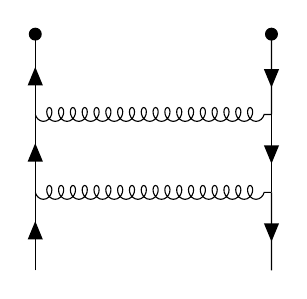
\begin{tikzpicture}[transform shape,scale=1,baseline=($(a)!0.5!(exa)$.base)]
			\begin{feynman}
				\node[dot] (a);
				\node[right=\FDWidth of a,dot] (b);
				\vertex[below=\FDHeight of a] (exa);
				\vertex[below=\FDHeight of b] (exb);
				% 
				\vertex at ($(a)!0.33!(b)$) (o13);
				\vertex at ($(a)!0.66!(b)$) (o23);
				\vertex at ($(a)!0.25!(b)$) (o14);
				\vertex at ($(a)!0.5!(b)$) (o12);
				\vertex at ($(a)!0.75!(b)$) (o34);
				% 
				\vertex at ($(a)!0.2!(b)$) (o15);
				\vertex at ($(a)!0.4!(b)$) (o25);
				\vertex at ($(a)!0.6!(b)$) (o35);
				\vertex at ($(a)!0.8!(b)$) (o45);
				% HOWTO: One can modify this to get vertexes lower than the gauge link line. 
				\vertex at ($(o13)+1/4*(0,-\FDHeight)$) (o13m);
				\vertex at ($(o23)+1/4*(0,-\FDHeight)$) (o23m);
				% 
				\vertex at ($(exa)!0.25!(a)$) (a14);
				\vertex at ($(exa)!0.5!(a)$) (a12);
				\vertex at ($(exa)!0.75!(a)$) (a34);
				\vertex at ($(exa)!0.33!(a)$) (a13);
				\vertex at ($(exa)!0.66!(a)$) (a23);
				% 
				\vertex at ($(exb)!0.25!(b)$) (b14);
				\vertex at ($(exb)!0.5!(b)$) (b12);
				\vertex at ($(exb)!0.75!(b)$) (b34);
				\vertex at ($(exb)!0.33!(b)$) (b13);
				\vertex at ($(exb)!0.66!(b)$) (b23);
				% 
				\vertex at ($(a12)!0.33!(b12)$) (ab13);
				\vertex at ($(a12)!0.66!(b12)$) (ab23);
				\vertex at ($(a12)!0.5!(b12)$) (ab12);
				% 
				\vertex at ($(a14)!0.5!(a34)!1.2!-90:(a34)$) (g1);
				% 
				\diagram*{
					(exa) --[fermion] (a13) --[fermion] (a23) --[fermion] (a);
					(b) --[fermion] (b23) --[fermion] (b13) --[fermion] (exb);
					(a13) --[gluon] (b13);
					(a23) --[gluon] (b23);
				};
			\end{feynman}
		\end{tikzpicture}
		\label{}
	}\hfil
	\subfloat[125]{
		\begin{tikzpicture}[transform shape,scale=1,baseline=($(a)!0.5!(exa)$.base)]
			\begin{feynman}
				\node[dot] (a);
				\node[right=\FDWidth of a,dot] (b);
				\vertex[below=\FDHeight of a] (exa);
				\vertex[below=\FDHeight of b] (exb);
				% 
				\vertex at ($(a)!0.33!(b)$) (o13);
				\vertex at ($(a)!0.66!(b)$) (o23);
				\vertex at ($(a)!0.25!(b)$) (o14);
				\vertex at ($(a)!0.5!(b)$) (o12);
				\vertex at ($(a)!0.75!(b)$) (o34);
				% 
				\vertex at ($(a)!0.2!(b)$) (o15);
				\vertex at ($(a)!0.4!(b)$) (o25);
				\vertex at ($(a)!0.6!(b)$) (o35);
				\vertex at ($(a)!0.8!(b)$) (o45);
				% 
				\vertex at ($(o13)+1/4*(0,-\FDHeight)$) (o13m);
				\vertex at ($(o23)+1/4*(0,-\FDHeight)$) (o23m);
				% 
				\vertex at ($(exa)!0.25!(a)$) (a14);
				\vertex at ($(exa)!0.5!(a)$) (a12);
				\vertex at ($(exa)!0.75!(a)$) (a34);
				\vertex at ($(exa)!0.33!(a)$) (a13);
				\vertex at ($(exa)!0.66!(a)$) (a23);
				% 
				\vertex at ($(exb)!0.25!(b)$) (b14);
				\vertex at ($(exb)!0.5!(b)$) (b12);
				\vertex at ($(exb)!0.75!(b)$) (b34);
				\vertex at ($(exb)!0.33!(b)$) (b13);
				\vertex at ($(exb)!0.66!(b)$) (b23);
				% 
				\vertex at ($(a12)!0.33!(b12)$) (ab13);
				\vertex at ($(a12)!0.66!(b12)$) (ab23);
				\vertex at ($(a12)!0.5!(b12)$) (ab12);
				% 
				\vertex at ($(a14)!0.5!(a34)!1.2!-90:(a34)$) (g1);
				% 
				\diagram*{
					(a) --[Eikonal] (o13);
					(o23) --[Eikonal] (b);
					(exa) --[fermion] (a);
					(b) --[fermion] (exb);
					(o13) --[gluon] (o13m);
					(o23) --[gluon] (o23m);
					(o13m) --[fermion] (o23m);
					(o23m) --[fermion,half left,looseness=1.5] (o13m);
				};
			\end{feynman}
		\end{tikzpicture}
		\label{}
	}\hfil
	\subfloat[128]{
		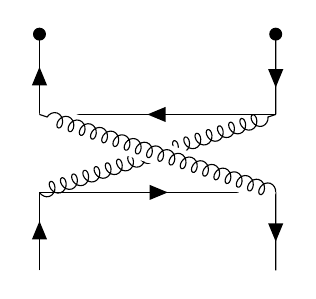
\begin{tikzpicture}[transform shape,scale=1,baseline=($(a)!0.5!(exa)$.base)]
			\begin{feynman}
				\node[dot] (a);
				\node[right=\FDWidth of a,dot] (b);
				\vertex[below=\FDHeight of a] (exa);
				\vertex[below=\FDHeight of b] (exb);
				% 
				\vertex at ($(a)!0.33!(b)$) (o13);
				\vertex at ($(a)!0.66!(b)$) (o23);
				\vertex at ($(a)!0.25!(b)$) (o14);
				\vertex at ($(a)!0.5!(b)$) (o12);
				\vertex at ($(a)!0.75!(b)$) (o34);
				% 
				\vertex at ($(a)!0.2!(b)$) (o15);
				\vertex at ($(a)!0.4!(b)$) (o25);
				\vertex at ($(a)!0.6!(b)$) (o35);
				\vertex at ($(a)!0.8!(b)$) (o45);
				% HOWTO: One can modify this to get vertexes lower than the gauge link line. 
				\vertex at ($(o13)+1/4*(0,-\FDHeight)$) (o13m);
				\vertex at ($(o23)+1/4*(0,-\FDHeight)$) (o23m);
				% 
				\vertex at ($(exa)!0.25!(a)$) (a14);
				\vertex at ($(exa)!0.5!(a)$) (a12);
				\vertex at ($(exa)!0.75!(a)$) (a34);
				\vertex at ($(exa)!0.33!(a)$) (a13);
				\vertex at ($(exa)!0.66!(a)$) (a23);
				% 
				\vertex at ($(exb)!0.25!(b)$) (b14);
				\vertex at ($(exb)!0.5!(b)$) (b12);
				\vertex at ($(exb)!0.75!(b)$) (b34);
				\vertex at ($(exb)!0.33!(b)$) (b13);
				\vertex at ($(exb)!0.66!(b)$) (b23);
				% 
				\vertex at ($(a12)!0.33!(b12)$) (ab13);
				\vertex at ($(a12)!0.66!(b12)$) (ab23);
				\vertex at ($(a12)!0.5!(b12)$) (ab12);
				% 
				\vertex at ($(a14)!0.5!(a34)!1.2!-90:(a34)$) (g1);
				% 
				\diagram*{
					(exa) --[fermion] (a13) --[fermion] (b13) --[fermion] (exb);
					(b) --[fermion] (b23) --[fermion] (a23) --[fermion] (a);
					(a13) --[gluon] (b23);
					(b13) --[white,line width=3mm] (a23);
					(b13) --[gluon] (a23);
				};
			\end{feynman}
		\end{tikzpicture}
		\label{}
	}\hfil
	\subfloat[133]{
		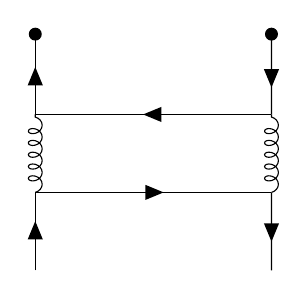
\begin{tikzpicture}[transform shape,scale=1,baseline=($(a)!0.5!(exa)$.base)]
			\begin{feynman}
				\node[dot] (a);
				\node[right=\FDWidth of a,dot] (b);
				\vertex[below=\FDHeight of a] (exa);
				\vertex[below=\FDHeight of b] (exb);
				% 
				\vertex at ($(a)!0.33!(b)$) (o13);
				\vertex at ($(a)!0.66!(b)$) (o23);
				\vertex at ($(a)!0.25!(b)$) (o14);
				\vertex at ($(a)!0.5!(b)$) (o12);
				\vertex at ($(a)!0.75!(b)$) (o34);
				% 
				\vertex at ($(a)!0.2!(b)$) (o15);
				\vertex at ($(a)!0.4!(b)$) (o25);
				\vertex at ($(a)!0.6!(b)$) (o35);
				\vertex at ($(a)!0.8!(b)$) (o45);
				% HOWTO: One can modify this to get vertexes lower than the gauge link line. 
				\vertex at ($(o13)+1/4*(0,-\FDHeight)$) (o13m);
				\vertex at ($(o23)+1/4*(0,-\FDHeight)$) (o23m);
				% 
				\vertex at ($(exa)!0.25!(a)$) (a14);
				\vertex at ($(exa)!0.5!(a)$) (a12);
				\vertex at ($(exa)!0.75!(a)$) (a34);
				\vertex at ($(exa)!0.33!(a)$) (a13);
				\vertex at ($(exa)!0.66!(a)$) (a23);
				% 
				\vertex at ($(exb)!0.25!(b)$) (b14);
				\vertex at ($(exb)!0.5!(b)$) (b12);
				\vertex at ($(exb)!0.75!(b)$) (b34);
				\vertex at ($(exb)!0.33!(b)$) (b13);
				\vertex at ($(exb)!0.66!(b)$) (b23);
				% 
				\vertex at ($(a12)!0.33!(b12)$) (ab13);
				\vertex at ($(a12)!0.66!(b12)$) (ab23);
				\vertex at ($(a12)!0.5!(b12)$) (ab12);
				% 
				\vertex at ($(a14)!0.5!(a34)!1.2!-90:(a34)$) (g1);
				% 
				\diagram*{
					(exa) --[fermion] (a13) --[fermion] (b13) --[fermion] (exb);
					(b) --[fermion] (b23) --[fermion] (a23) --[fermion] (a);
					(a13) --[gluon] (a23);
					(b13) --[gluon] (b23);
				};
			\end{feynman}
		\end{tikzpicture}
		\label{}
	}\hfil\null\\\null\hfil
	\subfloat[143]{
		\begin{tikzpicture}[transform shape,scale=1,baseline=($(a)!0.5!(exa)$.base)]
			\begin{feynman}
				\node[dot] (a);
				\node[right=\FDWidth of a,dot] (b);
				\vertex[below=\FDHeight of a] (exa);
				\vertex[below=\FDHeight of b] (exb);
				% 
				\vertex at ($(a)!0.33!(b)$) (o13);
				\vertex at ($(a)!0.66!(b)$) (o23);
				\vertex at ($(a)!0.25!(b)$) (o14);
				\vertex at ($(a)!0.5!(b)$) (o12);
				\vertex at ($(a)!0.75!(b)$) (o34);
				% 
				\vertex at ($(a)!0.2!(b)$) (o15);
				\vertex at ($(a)!0.4!(b)$) (o25);
				\vertex at ($(a)!0.6!(b)$) (o35);
				\vertex at ($(a)!0.8!(b)$) (o45);
				% HOWTO: One can modify this to get vertexes lower than the gauge link line. 
				\vertex at ($(o13)+1/4*(0,-\FDHeight)$) (o13m);
				\vertex at ($(o23)+1/4*(0,-\FDHeight)$) (o23m);
				% 
				\vertex at ($(exa)!0.25!(a)$) (a14);
				\vertex at ($(exa)!0.5!(a)$) (a12);
				\vertex at ($(exa)!0.75!(a)$) (a34);
				\vertex at ($(exa)!0.33!(a)$) (a13);
				\vertex at ($(exa)!0.66!(a)$) (a23);
				% 
				\vertex at ($(exb)!0.25!(b)$) (b14);
				\vertex at ($(exb)!0.5!(b)$) (b12);
				\vertex at ($(exb)!0.75!(b)$) (b34);
				\vertex at ($(exb)!0.33!(b)$) (b13);
				\vertex at ($(exb)!0.66!(b)$) (b23);
				% 
				\vertex at ($(a12)!0.33!(b12)$) (ab13);
				\vertex at ($(a12)!0.66!(b12)$) (ab23);
				\vertex at ($(a12)!0.5!(b12)$) (ab12);
				% 
				\vertex at ($(o12)!1.3!-90:(o23)$) (g1);
				\vertex at ($(g1)+1/4*(0,-\FDHeight)$) (gtad);
				% 
				\diagram*{
					(a) --[Eikonal] (o13);
					(o23) --[Eikonal] (b);
					(exa) --[fermion] (a);
					(b) --[fermion] (exb);
					(o13) --[gluon,half right] (o23);
					(g1) --[gluon,out=-135,in=180] (gtad) --[gluon,out=0,in=-45] (g1);
				};
			\end{feynman}
		\end{tikzpicture}
		\label{}
	}\hfil
	\subfloat[144]{
		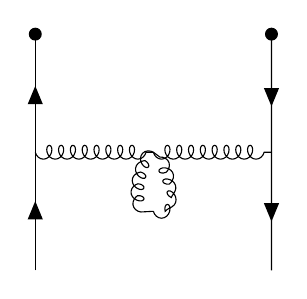
\begin{tikzpicture}[transform shape,scale=1,baseline=($(a)!0.5!(exa)$.base)]
			\begin{feynman}
				\node[dot] (a);
				\node[right=\FDWidth of a,dot] (b);
				\vertex[below=\FDHeight of a] (exa);
				\vertex[below=\FDHeight of b] (exb);
				% 
				\vertex at ($(a)!0.33!(b)$) (o13);
				\vertex at ($(a)!0.66!(b)$) (o23);
				\vertex at ($(a)!0.25!(b)$) (o14);
				\vertex at ($(a)!0.5!(b)$) (o12);
				\vertex at ($(a)!0.75!(b)$) (o34);
				% 
				\vertex at ($(a)!0.2!(b)$) (o15);
				\vertex at ($(a)!0.4!(b)$) (o25);
				\vertex at ($(a)!0.6!(b)$) (o35);
				\vertex at ($(a)!0.8!(b)$) (o45);
				% HOWTO: One can modify this to get vertexes lower than the gauge link line. 
				\vertex at ($(o13)+1/4*(0,-\FDHeight)$) (o13m);
				\vertex at ($(o23)+1/4*(0,-\FDHeight)$) (o23m);
				% 
				\vertex at ($(exa)!0.25!(a)$) (a14);
				\vertex at ($(exa)!0.5!(a)$) (a12);
				\vertex at ($(exa)!0.75!(a)$) (a34);
				\vertex at ($(exa)!0.33!(a)$) (a13);
				\vertex at ($(exa)!0.66!(a)$) (a23);
				% 
				\vertex at ($(exb)!0.25!(b)$) (b14);
				\vertex at ($(exb)!0.5!(b)$) (b12);
				\vertex at ($(exb)!0.75!(b)$) (b34);
				\vertex at ($(exb)!0.33!(b)$) (b13);
				\vertex at ($(exb)!0.66!(b)$) (b23);
				% 
				\vertex at ($(a12)!0.33!(b12)$) (ab13);
				\vertex at ($(a12)!0.66!(b12)$) (ab23);
				\vertex at ($(a12)!0.5!(b12)$) (ab12);
				% 
				\vertex at ($(ab12)+1/4*(0,-\FDHeight)$) (gtad);
				% 
				\diagram*{
					(exa) --[fermion] (a12) --[fermion] (a);
					(b) --[fermion] (b12) --[fermion] (exb);
					(a12) --[gluon] (ab12) --[gluon] (b12);
					(ab12) --[gluon,out=-135,in=180] (gtad) --[gluon,out=0,in=-45] (ab12);
				};
			\end{feynman}
		\end{tikzpicture}
		\label{}
	}\hfil\null
	\caption{All self-conjugated diagrams. }
	\label{re:sc}
\end{figure}
\begin{figure}[!htbp]
	\centering\null\hfil
	\subfloat[2]{
		\centering
		\begin{tikzpicture}[transform shape,scale=1,baseline=($(a)!0.5!(exa)$.base)]
			\begin{feynman}
				\node[dot] (a);
				\node[right=\FDWidth of a,dot] (b);
				\vertex[below=\FDHeight of a] (exa);
				\vertex[below=\FDHeight of b] (exb);
				% 
				\vertex at ($(a)!0.33!(b)$) (o13);
				\vertex at ($(a)!0.66!(b)$) (o23);
				\vertex at ($(a)!0.25!(b)$) (o14);
				\vertex at ($(a)!0.5!(b)$) (o12);
				\vertex at ($(a)!0.75!(b)$) (o34);
				% 
				\vertex at ($(exa)!0.25!(a)$) (a14);
				\vertex at ($(exa)!0.5!(a)$) (a12);
				\vertex at ($(exa)!0.75!(a)$) (a34);
				% 
				\vertex at ($(exb)!0.25!(b)$) (b14);
				\vertex at ($(exb)!0.5!(b)$) (b12);
				\vertex at ($(exb)!0.75!(b)$) (b34);
				% 
				\vertex at ($(a12)!0.33!(b12)$) (ab13);
				\vertex at ($(a12)!0.66!(b12)$) (ab23);
				\vertex at ($(a12)!0.5!(b12)$) (ab12);
				% 
				\vertex at ($(a14)!0.5!(a34)!1.2!-90:(a34)$) (g1);
				\vertex at ($(a12)!0.5!(o23)$) (g2);
				% 
				\diagram*{
					(a) --[Eikonal] (o13);
					(o23) --[Eikonal] (b);
					(exa) --[fermion] (a12) --[fermion] (a);
					(b) --[fermion] (exb);
					(o13) --[gluon] (ab13) --[gluon] (a12);
					(o23) --[gluon] (ab13);
				};
			\end{feynman}
		\end{tikzpicture}
		\label{}
	}\hfil
	\subfloat[3]{
		\centering
		\begin{tikzpicture}[transform shape,scale=1,baseline=($(a)!0.5!(exa)$.base)]
			\begin{feynman}
				\node[dot] (a);
				\node[right=\FDWidth of a,dot] (b);
				\vertex[below=\FDHeight of a] (exa);
				\vertex[below=\FDHeight of b] (exb);
				% 
				\vertex at ($(a)!0.33!(b)$) (o13);
				\vertex at ($(a)!0.66!(b)$) (o23);
				\vertex at ($(a)!0.25!(b)$) (o14);
				\vertex at ($(a)!0.5!(b)$) (o12);
				\vertex at ($(a)!0.75!(b)$) (o34);
				% 
				\vertex at ($(exa)!0.25!(a)$) (a14);
				\vertex at ($(exa)!0.5!(a)$) (a12);
				\vertex at ($(exa)!0.75!(a)$) (a34);
				% 
				\vertex at ($(exb)!0.25!(b)$) (b14);
				\vertex at ($(exb)!0.5!(b)$) (b12);
				\vertex at ($(exb)!0.75!(b)$) (b34);
				% 
				\vertex at ($(a12)!0.33!(b12)$) (ab13);
				\vertex at ($(a12)!0.66!(b12)$) (ab23);
				\vertex at ($(a12)!0.5!(b12)$) (ab12);
				% 
				\vertex at ($(a14)!0.5!(a34)!1.2!-90:(a34)$) (g1);
				% 
				\diagram*{
					(a) --[Eikonal] (o12);
					(exa) --[fermion] (a12) --[fermion] (a);
					(b) --[fermion] (b12) --[fermion] (exb);
					(o12) --[gluon] (ab12);
					(a12) --[gluon] (ab12) --[gluon] (b12);
				};
			\end{feynman}
		\end{tikzpicture}
		\label{}
	}\hfil
	\subfloat[85]{
		\begin{tikzpicture}[transform shape,scale=1,baseline=($(a)!0.5!(exa)$.base)]
			\begin{feynman}
				\node[dot] (a);
				\node[right=\FDWidth of a,dot] (b);
				\vertex[below=\FDHeight of a] (exa);
				\vertex[below=\FDHeight of b] (exb);
				% 
				\vertex at ($(a)!0.33!(b)$) (o13);
				\vertex at ($(a)!0.66!(b)$) (o23);
				\vertex at ($(a)!0.25!(b)$) (o14);
				\vertex at ($(a)!0.5!(b)$) (o12);
				\vertex at ($(a)!0.75!(b)$) (o34);
				% 
				\vertex at ($(exa)!0.25!(a)$) (a14);
				\vertex at ($(exa)!0.5!(a)$) (a12);
				\vertex at ($(exa)!0.75!(a)$) (a34);
				% 
				\vertex at ($(exb)!0.25!(b)$) (b14);
				\vertex at ($(exb)!0.5!(b)$) (b12);
				\vertex at ($(exb)!0.75!(b)$) (b34);
				% 
				\vertex at ($(a12)!0.33!(b12)$) (ab13);
				\vertex at ($(a12)!0.66!(b12)$) (ab23);
				\vertex at ($(a12)!0.5!(b12)$) (ab12);
				% 
				\vertex at ($(a14)!0.5!(a34)!1.2!-90:(a34)$) (g1);
				% 
				\diagram*{
					(o13) --[Eikonal] (o23) --[Eikonal] (b);
					(exa) --[fermion] (a12) --[fermion] (a);
					(b) --[fermion] (exb);
					(o13) --[gluon] (ab13) --[gluon] (a12);
					(ab13) --[gluon] (o23);
				};
			\end{feynman}
		\end{tikzpicture}
		\label{}
	}\hfil
	\subfloat[5]{
		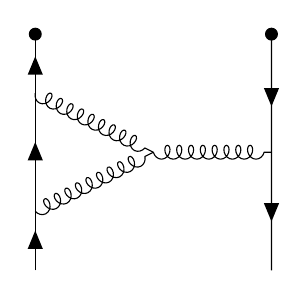
\begin{tikzpicture}[transform shape,scale=1,baseline=($(a)!0.5!(exa)$.base)]
			\begin{feynman}
				\node[dot] (a);
				\node[right=\FDWidth of a,dot] (b);
				\vertex[below=\FDHeight of a] (exa);
				\vertex[below=\FDHeight of b] (exb);
				% 
				\vertex at ($(a)!0.33!(b)$) (o13);
				\vertex at ($(a)!0.66!(b)$) (o23);
				\vertex at ($(a)!0.25!(b)$) (o14);
				\vertex at ($(a)!0.5!(b)$) (o12);
				\vertex at ($(a)!0.75!(b)$) (o34);
				% 
				\vertex at ($(exa)!0.25!(a)$) (a14);
				\vertex at ($(exa)!0.5!(a)$) (a12);
				\vertex at ($(exa)!0.75!(a)$) (a34);
				% 
				\vertex at ($(exb)!0.25!(b)$) (b14);
				\vertex at ($(exb)!0.5!(b)$) (b12);
				\vertex at ($(exb)!0.75!(b)$) (b34);
				% 
				\vertex at ($(a12)!0.33!(b12)$) (ab13);
				\vertex at ($(a12)!0.66!(b12)$) (ab23);
				\vertex at ($(a12)!0.5!(b12)$) (ab12);
				% 
				\vertex at ($(a14)!0.5!(a34)!1.2!-90:(a34)$) (g1);
				% 
				\diagram*{
					(exa) --[fermion] (a14) --[fermion] (a34) --[fermion] (a);
					(b) --[fermion] (b12) --[fermion] (exb);
					(a14) --[gluon] (ab12) --[gluon] (b12);
					(a34) --[gluon] (ab12);
				};
			\end{feynman}
		\end{tikzpicture}
		\label{}
	}\hfil\null\null\\\hfil
	\subfloat[6]{
		\begin{tikzpicture}[transform shape,scale=1,baseline=($(a)!0.5!(exa)$.base)]
			\begin{feynman}
				\node[dot] (a);
				\node[right=\FDWidth of a,dot] (b);
				\vertex[below=\FDHeight of a] (exa);
				\vertex[below=\FDHeight of b] (exb);
				% 
				\vertex at ($(a)!0.33!(b)$) (o13);
				\vertex at ($(a)!0.66!(b)$) (o23);
				\vertex at ($(a)!0.25!(b)$) (o14);
				\vertex at ($(a)!0.5!(b)$) (o12);
				\vertex at ($(a)!0.75!(b)$) (o34);
				% 
				\vertex at ($(exa)!0.25!(a)$) (a14);
				\vertex at ($(exa)!0.5!(a)$) (a12);
				\vertex at ($(exa)!0.75!(a)$) (a34);
				% 
				\vertex at ($(exb)!0.25!(b)$) (b14);
				\vertex at ($(exb)!0.5!(b)$) (b12);
				\vertex at ($(exb)!0.75!(b)$) (b34);
				% 
				\vertex at ($(a12)!0.33!(b12)$) (ab13);
				\vertex at ($(a12)!0.66!(b12)$) (ab23);
				\vertex at ($(a12)!0.5!(b12)$) (ab12);
				% 
				\vertex at ($(a14)!0.5!(a34)!1.2!-90:(a34)$) (g1);
				\vertex[above=10pt of ab12] (ab123);
				% 
				\diagram*{
					(a) --[Eikonal] (o14) --[Eikonal] (o12);
					(o34) --[Eikonal] (b);
					(exa) --[fermion] (a);
					(b) --[fermion] (exb);
					(o14) --[gluon, quarter right] (ab123);
					(o12) --[gluon] (ab123);
					(o34) --[gluon, quarter left] (ab123);
				};
			\end{feynman}
		\end{tikzpicture}
		\label{}
	}\hfil
	\subfloat[13]{
		\begin{tikzpicture}[transform shape,scale=1,baseline=($(a)!0.5!(exa)$.base)]
			\begin{feynman}
				\node[dot] (a);
				\node[right=\FDWidth of a,dot] (b);
				\vertex[below=\FDHeight of a] (exa);
				\vertex[below=\FDHeight of b] (exb);
				% 
				\vertex at ($(a)!0.33!(b)$) (o13);
				\vertex at ($(a)!0.66!(b)$) (o23);
				\vertex at ($(a)!0.25!(b)$) (o14);
				\vertex at ($(a)!0.5!(b)$) (o12);
				\vertex at ($(a)!0.75!(b)$) (o34);
				% 
				\vertex at ($(exa)!0.25!(a)$) (a14);
				\vertex at ($(exa)!0.5!(a)$) (a12);
				\vertex at ($(exa)!0.75!(a)$) (a34);
				% 
				\vertex at ($(exb)!0.25!(b)$) (b14);
				\vertex at ($(exb)!0.5!(b)$) (b12);
				\vertex at ($(exb)!0.75!(b)$) (b34);
				% 
				\vertex at ($(a12)!0.33!(b12)$) (ab13);
				\vertex at ($(a12)!0.66!(b12)$) (ab23);
				\vertex at ($(a12)!0.5!(b12)$) (ab12);
				% 
				\vertex at ($(a14)!0.5!(a34)!1.2!-90:(a34)$) (g1);
				\vertex at ($(o12)!0.66!(a12)$) (g13);
				\vertex at ($(o12)!0.33!(a12)$) (g23);
				% 
				\diagram*{
					(o12) --[Eikonal] (b);
					(exa) --[fermion] (a12) --[fermion] (a);
					(b) --[fermion] (exb);
					(a12) --[gluon] (g13);
					(g13) --[gluon] (g23);
					(g23) --[gluon] (o12);
					(g13) --[gluon,half right] (g23);
				};
			\end{feynman}
		\end{tikzpicture}
		\label{}
	}\hfil
	\subfloat[16]{
		\begin{tikzpicture}[transform shape,scale=1,baseline=($(a)!0.5!(exa)$.base)]
			\begin{feynman}
				\node[dot] (a);
				\node[right=\FDWidth of a,dot] (b);
				\vertex[below=\FDHeight of a] (exa);
				\vertex[below=\FDHeight of b] (exb);
				% 
				\vertex at ($(a)!0.33!(b)$) (o13);
				\vertex at ($(a)!0.66!(b)$) (o23);
				\vertex at ($(a)!0.25!(b)$) (o14);
				\vertex at ($(a)!0.5!(b)$) (o12);
				\vertex at ($(a)!0.75!(b)$) (o34);
				% 
				\vertex at ($(exa)!0.25!(a)$) (a14);
				\vertex at ($(exa)!0.5!(a)$) (a12);
				\vertex at ($(exa)!0.75!(a)$) (a34);
				% 
				\vertex at ($(exb)!0.25!(b)$) (b14);
				\vertex at ($(exb)!0.5!(b)$) (b12);
				\vertex at ($(exb)!0.75!(b)$) (b34);
				% 
				\vertex at ($(a12)!0.33!(b12)$) (ab13);
				\vertex at ($(a12)!0.66!(b12)$) (ab23);
				\vertex at ($(a12)!0.5!(b12)$) (ab12);
				% 
				\vertex at ($(a14)!0.5!(a34)!1.2!-90:(a34)$) (g1);
				% 
				\diagram*{
					(o12) --[Eikonal] (b);
					(exa) --[fermion] (a14) --[fermion] (a34) --[fermion] (a);
					(b) --[fermion] (exb);
					(a14) --[gluon] (ab12);
					(a34) --[gluon] (ab12);
					(o12) --[gluon] (ab12);
				};
			\end{feynman}
		\end{tikzpicture}
		\label{}
	}\hfil
	\subfloat[25]{
		\begin{tikzpicture}[transform shape,scale=1,baseline=($(a)!0.5!(exa)$.base)]
			\begin{feynman}
				\node[dot] (a);
				\node[right=\FDWidth of a,dot] (b);
				\vertex[below=\FDHeight of a] (exa);
				\vertex[below=\FDHeight of b] (exb);
				% 
				\vertex at ($(a)!0.33!(b)$) (o13);
				\vertex at ($(a)!0.66!(b)$) (o23);
				\vertex at ($(a)!0.25!(b)$) (o14);
				\vertex at ($(a)!0.5!(b)$) (o12);
				\vertex at ($(a)!0.75!(b)$) (o34);
				% 
				\vertex at ($(exa)!0.25!(a)$) (a14);
				\vertex at ($(exa)!0.5!(a)$) (a12);
				\vertex at ($(exa)!0.75!(a)$) (a34);
				% 
				\vertex at ($(exb)!0.25!(b)$) (b14);
				\vertex at ($(exb)!0.5!(b)$) (b12);
				\vertex at ($(exb)!0.75!(b)$) (b34);
				% 
				\vertex at ($(a12)!0.33!(b12)$) (ab13);
				\vertex at ($(a12)!0.66!(b12)$) (ab23);
				\vertex at ($(a12)!0.5!(b12)$) (ab12);
				% 
				\vertex at ($(a14)!0.5!(a34)!1.2!-90:(a34)$) (g1);
				\vertex at ($(o12)!0.66!(a12)$) (g13);
				\vertex at ($(o12)!0.33!(a12)$) (g23);
				% 
				\diagram*{
					(o12) --[Eikonal] (b);
					(exa) --[fermion] (a12) --[fermion] (a);
					(b) --[fermion] (exb);
					(a12) --[gluon] (g13);
					(g13) --[ghost] (g23);
					(g23) --[gluon] (o12);
					(g13) --[ghost,half right] (g23);
				};
			\end{feynman}
		\end{tikzpicture}
		\label{}
	}\hfil\null\\\null\hfil
	\subfloat[88]{
		\begin{tikzpicture}[transform shape,scale=1,baseline=($(a)!0.5!(exa)$.base)]
			\begin{feynman}
				\node[dot] (a);
				\node[right=\FDWidth of a,dot] (b);
				\vertex[below=\FDHeight of a] (exa);
				\vertex[below=\FDHeight of b] (exb);
				% 
				\vertex at ($(a)!0.33!(b)$) (o13);
				\vertex at ($(a)!0.66!(b)$) (o23);
				\vertex at ($(a)!0.25!(b)$) (o14);
				\vertex at ($(a)!0.5!(b)$) (o12);
				\vertex at ($(a)!0.75!(b)$) (o34);
				% 
				\vertex at ($(exa)!0.25!(a)$) (a14);
				\vertex at ($(exa)!0.5!(a)$) (a12);
				\vertex at ($(exa)!0.75!(a)$) (a34);
				\vertex at ($(exa)!0.33!(a)$) (a13);
				\vertex at ($(exa)!0.66!(a)$) (a23);
				% 
				\vertex at ($(exb)!0.25!(b)$) (b14);
				\vertex at ($(exb)!0.5!(b)$) (b12);
				\vertex at ($(exb)!0.75!(b)$) (b34);
				% 
				\vertex at ($(a12)!0.33!(b12)$) (ab13);
				\vertex at ($(a12)!0.66!(b12)$) (ab23);
				\vertex at ($(a12)!0.5!(b12)$) (ab12);
				% 
				\vertex at ($(a14)!0.5!(a34)!1.2!-90:(a34)$) (g1);
				% 
				\diagram*{
					(o13) --[Eikonal] (o23) --[Eikonal] (b);
					(exa) --[fermion] (a13) --[fermion] (a23) --[fermion] (a);
					(b) --[fermion] (exb);
					(a23) --[gluon] (o13);
					(a13) --[gluon] (o23);
				};
			\end{feynman}
		\end{tikzpicture}
		\label{}
	}\hfil
	\subfloat[31]{
		\begin{tikzpicture}[transform shape,scale=1,baseline=($(a)!0.5!(exa)$.base)]
			\begin{feynman}
				\node[dot] (a);
				\node[right=\FDWidth of a,dot] (b);
				\vertex[below=\FDHeight of a] (exa);
				\vertex[below=\FDHeight of b] (exb);
				% 
				\vertex at ($(a)!0.33!(b)$) (o13);
				\vertex at ($(a)!0.66!(b)$) (o23);
				\vertex at ($(a)!0.25!(b)$) (o14);
				\vertex at ($(a)!0.5!(b)$) (o12);
				\vertex at ($(a)!0.75!(b)$) (o34);
				% 
				\vertex at ($(exa)!0.25!(a)$) (a14);
				\vertex at ($(exa)!0.5!(a)$) (a12);
				\vertex at ($(exa)!0.75!(a)$) (a34);
				\vertex at ($(exa)!0.33!(a)$) (a13);
				\vertex at ($(exa)!0.66!(a)$) (a23);
				% 
				\vertex at ($(exb)!0.25!(b)$) (b14);
				\vertex at ($(exb)!0.5!(b)$) (b12);
				\vertex at ($(exb)!0.75!(b)$) (b34);
				% 
				\vertex at ($(a12)!0.33!(b12)$) (ab13);
				\vertex at ($(a12)!0.66!(b12)$) (ab23);
				\vertex at ($(a12)!0.5!(b12)$) (ab12);
				% 
				\vertex at ($(a14)!0.5!(a34)!1.2!-90:(a34)$) (g1);
				% 
				\diagram*{
					(a) --[Eikonal] (o13);
					(o23) --[Eikonal] (b);
					(exa) --[fermion] (a13) --[fermion] (a23) --[fermion] (a);
					(b) --[fermion] (exb);
					(a23) --[gluon] (o13);
					(a13) --[gluon] (o23);
				};
			\end{feynman}
		\end{tikzpicture}
		\label{}
	}\hfil
	\subfloat[32]{
		\begin{tikzpicture}[transform shape,scale=1,baseline=($(a)!0.5!(exa)$.base)]
			\begin{feynman}
				\node[dot] (a);
				\node[right=\FDWidth of a,dot] (b);
				\vertex[below=\FDHeight of a] (exa);
				\vertex[below=\FDHeight of b] (exb);
				% 
				\vertex at ($(a)!0.33!(b)$) (o13);
				\vertex at ($(a)!0.66!(b)$) (o23);
				\vertex at ($(a)!0.25!(b)$) (o14);
				\vertex at ($(a)!0.5!(b)$) (o12);
				\vertex at ($(a)!0.75!(b)$) (o34);
				% 
				\vertex at ($(exa)!0.25!(a)$) (a14);
				\vertex at ($(exa)!0.5!(a)$) (a12);
				\vertex at ($(exa)!0.75!(a)$) (a34);
				\vertex at ($(exa)!0.33!(a)$) (a13);
				\vertex at ($(exa)!0.66!(a)$) (a23);
				% 
				\vertex at ($(exb)!0.25!(b)$) (b14);
				\vertex at ($(exb)!0.5!(b)$) (b12);
				\vertex at ($(exb)!0.75!(b)$) (b34);
				\vertex at ($(exb)!0.33!(b)$) (b13);
				\vertex at ($(exb)!0.66!(b)$) (b23);
				% 
				\vertex at ($(a12)!0.33!(b12)$) (ab13);
				\vertex at ($(a12)!0.66!(b12)$) (ab23);
				\vertex at ($(a12)!0.5!(b12)$) (ab12);
				% 
				\vertex at ($(a14)!0.5!(a34)!1.2!-90:(a34)$) (g1);
				% 
				\diagram*{
					(a) --[Eikonal] (o13);
					(exa) --[fermion] (a13) --[fermion] (a23) --[fermion] (a);
					(b)  --[fermion] (b13)--[fermion] (exb);
					(a23) --[gluon] (o13);
					(a13) --[gluon] (b13);
				};
			\end{feynman}
		\end{tikzpicture}
		\label{}
	}\hfil
	\subfloat[38]{
		\begin{tikzpicture}[transform shape,scale=1,baseline=($(a)!0.5!(exa)$.base)]
			\begin{feynman}
				\node[dot] (a);
				\node[right=\FDWidth of a,dot] (b);
				\vertex[below=\FDHeight of a] (exa);
				\vertex[below=\FDHeight of b] (exb);
				% 
				\vertex at ($(a)!0.33!(b)$) (o13);
				\vertex at ($(a)!0.66!(b)$) (o23);
				\vertex at ($(a)!0.25!(b)$) (o14);
				\vertex at ($(a)!0.5!(b)$) (o12);
				\vertex at ($(a)!0.75!(b)$) (o34);
				% 
				\vertex at ($(exa)!0.25!(a)$) (a14);
				\vertex at ($(exa)!0.5!(a)$) (a12);
				\vertex at ($(exa)!0.75!(a)$) (a34);
				\vertex at ($(exa)!0.33!(a)$) (a13);
				\vertex at ($(exa)!0.66!(a)$) (a23);
				% 
				\vertex at ($(exb)!0.25!(b)$) (b14);
				\vertex at ($(exb)!0.5!(b)$) (b12);
				\vertex at ($(exb)!0.75!(b)$) (b34);
				% 
				\vertex at ($(a12)!0.33!(b12)$) (ab13);
				\vertex at ($(a12)!0.66!(b12)$) (ab23);
				\vertex at ($(a12)!0.5!(b12)$) (ab12);
				% 
				\vertex at ($(a14)!0.5!(a34)!1.2!-90:(a34)$) (g1);
				% 
				\diagram*{
					(a) --[Eikonal] (o14);
					(o12) --[Eikonal] (o34) --[Eikonal] (b);
					(exa) --[fermion] (a12) --[fermion] (a);
					(b) --[fermion] (exb);
					(a12) --[gluon] (o12);
					(o34) --[gluon,half right,looseness=1.5] (o14);
				};
			\end{feynman}
		\end{tikzpicture}
		\label{}
	}\hfil\null\\\null\hfil
	\subfloat[89]{
		\begin{tikzpicture}[transform shape,scale=1,baseline=($(a)!0.5!(exa)$.base)]
			\begin{feynman}
				\node[dot] (a);
				\node[right=\FDWidth of a,dot] (b);
				\vertex[below=\FDHeight of a] (exa);
				\vertex[below=\FDHeight of b] (exb);
				% 
				\vertex at ($(a)!0.33!(b)$) (o13);
				\vertex at ($(a)!0.66!(b)$) (o23);
				\vertex at ($(a)!0.25!(b)$) (o14);
				\vertex at ($(a)!0.5!(b)$) (o12);
				\vertex at ($(a)!0.75!(b)$) (o34);
				% 
				\vertex at ($(exa)!0.25!(a)$) (a14);
				\vertex at ($(exa)!0.5!(a)$) (a12);
				\vertex at ($(exa)!0.75!(a)$) (a34);
				\vertex at ($(exa)!0.33!(a)$) (a13);
				\vertex at ($(exa)!0.66!(a)$) (a23);
				% 
				\vertex at ($(exb)!0.25!(b)$) (b14);
				\vertex at ($(exb)!0.5!(b)$) (b12);
				\vertex at ($(exb)!0.75!(b)$) (b34);
				\vertex at ($(exb)!0.33!(b)$) (b13);
				\vertex at ($(exb)!0.66!(b)$) (b23);
				% 
				\vertex at ($(a12)!0.33!(b12)$) (ab13);
				\vertex at ($(a12)!0.66!(b12)$) (ab23);
				\vertex at ($(a12)!0.5!(b12)$) (ab12);
				% 
				\vertex at ($(a14)!0.5!(a34)!1.2!-90:(a34)$) (g1);
				% 
				\diagram*{
					(a) --[Eikonal] (o14);
					(o12)--[Eikonal] (o34) --[Eikonal] (b);
					(exa) --[fermion] (a12) --[fermion] (a);
					(b) --[fermion] (exb);
					(o14) --[gluon,half right] (o12);
					(a12) --[gluon,quarter right,looseness=0.8] (o34);
				};
			\end{feynman}
		\end{tikzpicture}
		\label{}
	}\hfil
	\subfloat[40]{
		\begin{tikzpicture}[transform shape,scale=1,baseline=($(a)!0.5!(exa)$.base)]
			\begin{feynman}
				\node[dot] (a);
				\node[right=\FDWidth of a,dot] (b);
				\vertex[below=\FDHeight of a] (exa);
				\vertex[below=\FDHeight of b] (exb);
				% 
				\vertex at ($(a)!0.33!(b)$) (o13);
				\vertex at ($(a)!0.66!(b)$) (o23);
				\vertex at ($(a)!0.25!(b)$) (o14);
				\vertex at ($(a)!0.5!(b)$) (o12);
				\vertex at ($(a)!0.75!(b)$) (o34);
				% 
				\vertex at ($(exa)!0.25!(a)$) (a14);
				\vertex at ($(exa)!0.5!(a)$) (a12);
				\vertex at ($(exa)!0.75!(a)$) (a34);
				\vertex at ($(exa)!0.33!(a)$) (a13);
				\vertex at ($(exa)!0.66!(a)$) (a23);
				% 
				\vertex at ($(exb)!0.25!(b)$) (b14);
				\vertex at ($(exb)!0.5!(b)$) (b12);
				\vertex at ($(exb)!0.75!(b)$) (b34);
				\vertex at ($(exb)!0.33!(b)$) (b13);
				\vertex at ($(exb)!0.66!(b)$) (b23);
				% 
				\vertex at ($(a12)!0.33!(b12)$) (ab13);
				\vertex at ($(a12)!0.66!(b12)$) (ab23);
				\vertex at ($(a12)!0.5!(b12)$) (ab12);
				% 
				\vertex at ($(a14)!0.5!(a34)!1.2!-90:(a34)$) (g1);
				% 
				\diagram*{
					(a) --[Eikonal] (o14) --[Eikonal] (o12) ;
					(o34) --[Eikonal] (b);
					(exa) --[fermion] (a12) --[fermion] (a);
					(b) --[fermion] (exb);
					(o12) --[gluon,half right] (o34);
					(a12) --[gluon] (o14);
				};
			\end{feynman}
		\end{tikzpicture}
		\label{}
	}\hfil
	\subfloat[74]{
		\begin{tikzpicture}[transform shape,scale=1,baseline=($(a)!0.5!(exa)$.base)]
			\begin{feynman}
				\node[dot] (a);
				\node[right=\FDWidth of a,dot] (b);
				\vertex[below=\FDHeight of a] (exa);
				\vertex[below=\FDHeight of b] (exb);
				% 
				\vertex at ($(a)!0.33!(b)$) (o13);
				\vertex at ($(a)!0.66!(b)$) (o23);
				\vertex at ($(a)!0.25!(b)$) (o14);
				\vertex at ($(a)!0.5!(b)$) (o12);
				\vertex at ($(a)!0.75!(b)$) (o34);
				% 
				\vertex at ($(exa)!0.25!(a)$) (a14);
				\vertex at ($(exa)!0.5!(a)$) (a12);
				\vertex at ($(exa)!0.75!(a)$) (a34);
				\vertex at ($(exa)!0.33!(a)$) (a13);
				\vertex at ($(exa)!0.66!(a)$) (a23);
				% 
				\vertex at ($(exb)!0.25!(b)$) (b14);
				\vertex at ($(exb)!0.5!(b)$) (b12);
				\vertex at ($(exb)!0.75!(b)$) (b34);
				\vertex at ($(exb)!0.33!(b)$) (b13);
				\vertex at ($(exb)!0.66!(b)$) (b23);
				% 
				\vertex at ($(a12)!0.33!(b12)$) (ab13);
				\vertex at ($(a12)!0.66!(b12)$) (ab23);
				\vertex at ($(a12)!0.5!(b12)$) (ab12);
				% 
				\vertex at ($(a14)!0.5!(a34)!1.2!-90:(a34)$) (g1);
				% 
				\diagram*{
					(o12) --[Eikonal] (b);
					(exa) --[fermion] (a13) --[fermion] (a23) --[fermion] (a);
					(b) --[fermion] (b23) --[fermion] (exb);
					(a23) --[gluon] (b23);
					(a13) --[white,line width=3mm] (o12);
					(a13) --[gluon] (o12);
				};
			\end{feynman}
		\end{tikzpicture}
		\label{}
	}\hfil
	\subfloat[54]{
		\begin{tikzpicture}[transform shape,scale=1,baseline=($(a)!0.5!(exa)$.base)]
			\begin{feynman}
				\node[dot] (a);
				\node[right=\FDWidth of a,dot] (b);
				\vertex[below=\FDHeight of a] (exa);
				\vertex[below=\FDHeight of b] (exb);
				% 
				\vertex at ($(a)!0.33!(b)$) (o13);
				\vertex at ($(a)!0.66!(b)$) (o23);
				\vertex at ($(a)!0.25!(b)$) (o14);
				\vertex at ($(a)!0.5!(b)$) (o12);
				\vertex at ($(a)!0.75!(b)$) (o34);
				% 
				\vertex at ($(a)!0.2!(b)$) (o15);
				\vertex at ($(a)!0.4!(b)$) (o25);
				\vertex at ($(a)!0.6!(b)$) (o35);
				\vertex at ($(a)!0.8!(b)$) (o45);
				% 
				\vertex at ($(exa)!0.25!(a)$) (a14);
				\vertex at ($(exa)!0.5!(a)$) (a12);
				\vertex at ($(exa)!0.75!(a)$) (a34);
				\vertex at ($(exa)!0.33!(a)$) (a13);
				\vertex at ($(exa)!0.66!(a)$) (a23);
				% 
				\vertex at ($(exb)!0.25!(b)$) (b14);
				\vertex at ($(exb)!0.5!(b)$) (b12);
				\vertex at ($(exb)!0.75!(b)$) (b34);
				\vertex at ($(exb)!0.33!(b)$) (b13);
				\vertex at ($(exb)!0.66!(b)$) (b23);
				% 
				\vertex at ($(a12)!0.33!(b12)$) (ab13);
				\vertex at ($(a12)!0.66!(b12)$) (ab23);
				\vertex at ($(a12)!0.5!(b12)$) (ab12);
				% 
				\vertex at ($(a14)!0.5!(a34)!1.2!-90:(a34)$) (g1);
				% 
				\diagram*{
					(a) --[Eikonal] (o15) --[Eikonal] (o25) --[Eikonal] (o35);
					(o45) --[Eikonal] (b);
					(exa) --[fermion] (a);
					(b) --[fermion] (exb);
					(o35) --[gluon,half right] (o45);
					(o15) --[gluon,half right] (o25);
				};
			\end{feynman}
		\end{tikzpicture}
		\label{}
	}\hfil\null\\\null\hfil
	\subfloat[81]{
		\begin{tikzpicture}[transform shape,scale=1,baseline=($(a)!0.5!(exa)$.base)]
			\begin{feynman}
				\node[dot] (a);
				\node[right=\FDWidth of a,dot] (b);
				\vertex[below=\FDHeight of a] (exa);
				\vertex[below=\FDHeight of b] (exb);
				% 
				\vertex at ($(a)!0.33!(b)$) (o13);
				\vertex at ($(a)!0.66!(b)$) (o23);
				\vertex at ($(a)!0.25!(b)$) (o14);
				\vertex at ($(a)!0.5!(b)$) (o12);
				\vertex at ($(a)!0.75!(b)$) (o34);
				% 
				\vertex at ($(a)!0.2!(b)$) (o15);
				\vertex at ($(a)!0.4!(b)$) (o25);
				\vertex at ($(a)!0.6!(b)$) (o35);
				\vertex at ($(a)!0.8!(b)$) (o45);
				% 
				\vertex at ($(exa)!0.25!(a)$) (a14);
				\vertex at ($(exa)!0.5!(a)$) (a12);
				\vertex at ($(exa)!0.75!(a)$) (a34);
				\vertex at ($(exa)!0.33!(a)$) (a13);
				\vertex at ($(exa)!0.66!(a)$) (a23);
				% 
				\vertex at ($(exb)!0.25!(b)$) (b14);
				\vertex at ($(exb)!0.5!(b)$) (b12);
				\vertex at ($(exb)!0.75!(b)$) (b34);
				\vertex at ($(exb)!0.33!(b)$) (b13);
				\vertex at ($(exb)!0.66!(b)$) (b23);
				% 
				\vertex at ($(a12)!0.33!(b12)$) (ab13);
				\vertex at ($(a12)!0.66!(b12)$) (ab23);
				\vertex at ($(a12)!0.5!(b12)$) (ab12);
				% 
				\vertex at ($(a14)!0.5!(a34)!1.2!-90:(a34)$) (g1);
				% 
				\diagram*{
					(o25) --[Eikonal] (o35) --[Eikonal] (o45) --[Eikonal] (b);
					(exa) --[fermion] (a12) --[fermion] (a);
					(b) --[fermion] (exb);
					(a12) --[gluon] (o25);
					(o35) --[gluon,half right] (o45);
				};
			\end{feynman}
		\end{tikzpicture}
		\label{}
	}\hfil
	\subfloat[84]{
		\begin{tikzpicture}[transform shape,scale=1,baseline=($(a)!0.5!(exa)$.base)]
			\begin{feynman}
				\node[dot] (a);
				\node[right=\FDWidth of a,dot] (b);
				\vertex[below=\FDHeight of a] (exa);
				\vertex[below=\FDHeight of b] (exb);
				% 
				\vertex at ($(a)!0.33!(b)$) (o13);
				\vertex at ($(a)!0.66!(b)$) (o23);
				\vertex at ($(a)!0.25!(b)$) (o14);
				\vertex at ($(a)!0.5!(b)$) (o12);
				\vertex at ($(a)!0.75!(b)$) (o34);
				% 
				\vertex at ($(a)!0.2!(b)$) (o15);
				\vertex at ($(a)!0.4!(b)$) (o25);
				\vertex at ($(a)!0.6!(b)$) (o35);
				\vertex at ($(a)!0.8!(b)$) (o45);
				% 
				\vertex at ($(exa)!0.25!(a)$) (a14);
				\vertex at ($(exa)!0.5!(a)$) (a12);
				\vertex at ($(exa)!0.75!(a)$) (a34);
				\vertex at ($(exa)!0.33!(a)$) (a13);
				\vertex at ($(exa)!0.66!(a)$) (a23);
				% 
				\vertex at ($(exb)!0.25!(b)$) (b14);
				\vertex at ($(exb)!0.5!(b)$) (b12);
				\vertex at ($(exb)!0.75!(b)$) (b34);
				\vertex at ($(exb)!0.33!(b)$) (b13);
				\vertex at ($(exb)!0.66!(b)$) (b23);
				% 
				\vertex at ($(a12)!0.33!(b12)$) (ab13);
				\vertex at ($(a12)!0.66!(b12)$) (ab23);
				\vertex at ($(a12)!0.5!(b12)$) (ab12);
				% 
				\vertex at ($(a14)!0.5!(a34)!1.2!-90:(a34)$) (g1);
				% 
				\diagram*{
					(o13) --[Eikonal] (o23) --[Eikonal] (b);
					(exa) --[fermion] (a12) --[fermion] (a);
					(b) --[fermion] (b12) --[fermion] (exb);
					(b12) --[gluon] (o23);
					(a12) --[gluon] (o13);
				};
			\end{feynman}
		\end{tikzpicture}
		\label{}
	}\hfil
	\subfloat[58]{
		\begin{tikzpicture}[transform shape,scale=1,baseline=($(a)!0.5!(exa)$.base)]
			\begin{feynman}
				\node[dot] (a);
				\node[right=\FDWidth of a,dot] (b);
				\vertex[below=\FDHeight of a] (exa);
				\vertex[below=\FDHeight of b] (exb);
				% 
				\vertex at ($(a)!0.33!(b)$) (o13);
				\vertex at ($(a)!0.66!(b)$) (o23);
				\vertex at ($(a)!0.25!(b)$) (o14);
				\vertex at ($(a)!0.5!(b)$) (o12);
				\vertex at ($(a)!0.75!(b)$) (o34);
				% 
				\vertex at ($(a)!0.2!(b)$) (o15);
				\vertex at ($(a)!0.4!(b)$) (o25);
				\vertex at ($(a)!0.6!(b)$) (o35);
				\vertex at ($(a)!0.8!(b)$) (o45);
				% 
				\vertex at ($(exa)!0.25!(a)$) (a14);
				\vertex at ($(exa)!0.5!(a)$) (a12);
				\vertex at ($(exa)!0.75!(a)$) (a34);
				\vertex at ($(exa)!0.33!(a)$) (a13);
				\vertex at ($(exa)!0.66!(a)$) (a23);
				% 
				\vertex at ($(exb)!0.25!(b)$) (b14);
				\vertex at ($(exb)!0.5!(b)$) (b12);
				\vertex at ($(exb)!0.75!(b)$) (b34);
				\vertex at ($(exb)!0.33!(b)$) (b13);
				\vertex at ($(exb)!0.66!(b)$) (b23);
				% 
				\vertex at ($(a12)!0.33!(b12)$) (ab13);
				\vertex at ($(a12)!0.66!(b12)$) (ab23);
				\vertex at ($(a12)!0.5!(b12)$) (ab12);
				% 
				\vertex at ($(a14)!0.5!(a34)!1.2!-90:(a34)$) (g1);
				% 
				\diagram*{
					(a) --[Eikonal] (o15) --[Eikonal] (o25) --[Eikonal] (o35);
					(o45) --[Eikonal] (b);
					(exa) --[fermion] (a);
					(b) --[fermion] (exb);
					(o25) --[gluon,half right] (o45);
					(o35) --[gluon,half right,looseness=1.5] (o15);
				};
			\end{feynman}
		\end{tikzpicture}
		\label{}
	}\hfil
	\subfloat[95]{
		\begin{tikzpicture}[transform shape,scale=1,baseline=($(a)!0.5!(exa)$.base)]
			\begin{feynman}
				\node[dot] (a);
				\node[right=\FDWidth of a,dot] (b);
				\vertex[below=\FDHeight of a] (exa);
				\vertex[below=\FDHeight of b] (exb);
				% 
				\vertex at ($(a)!0.33!(b)$) (o13);
				\vertex at ($(a)!0.66!(b)$) (o23);
				\vertex at ($(a)!0.25!(b)$) (o14);
				\vertex at ($(a)!0.5!(b)$) (o12);
				\vertex at ($(a)!0.75!(b)$) (o34);
				% 
				\vertex at ($(a)!0.2!(b)$) (o15);
				\vertex at ($(a)!0.4!(b)$) (o25);
				\vertex at ($(a)!0.6!(b)$) (o35);
				\vertex at ($(a)!0.8!(b)$) (o45);
				% 
				\vertex at ($(exa)!0.25!(a)$) (a14);
				\vertex at ($(exa)!0.5!(a)$) (a12);
				\vertex at ($(exa)!0.75!(a)$) (a34);
				\vertex at ($(exa)!0.33!(a)$) (a13);
				\vertex at ($(exa)!0.66!(a)$) (a23);
				% 
				\vertex at ($(exb)!0.25!(b)$) (b14);
				\vertex at ($(exb)!0.5!(b)$) (b12);
				\vertex at ($(exb)!0.75!(b)$) (b34);
				\vertex at ($(exb)!0.33!(b)$) (b13);
				\vertex at ($(exb)!0.66!(b)$) (b23);
				% 
				\vertex at ($(a12)!0.33!(b12)$) (ab13);
				\vertex at ($(a12)!0.66!(b12)$) (ab23);
				\vertex at ($(a12)!0.5!(b12)$) (ab12);
				% 
				\vertex at ($(a14)!0.5!(a34)!1.2!-90:(a34)$) (g1);
				% 
				\diagram*{
					(o14) --[Eikonal] (o12) --[Eikonal] (o34) --[Eikonal] (b);
					(exa) --[fermion] (a12) --[fermion] (a);
					(b) --[fermion] (exb);
					(a12) --[gluon] (o12);
					(o34) --[gluon,half right, looseness=1.5] (o14);
				};
			\end{feynman}
		\end{tikzpicture}
		\label{}
	}\hfil\null
	% 
	\caption{All real diagrams (excluding conjugated diagrams). }
	\label{re:c}
\end{figure}
\begin{figure}\ContinuedFloat
	\centering
	\null\hfil
	\subfloat[60]{
		\begin{tikzpicture}[transform shape,scale=1,baseline=($(a)!0.5!(exa)$.base)]
			\begin{feynman}
				\node[dot] (a);
				\node[right=\FDWidth of a,dot] (b);
				\vertex[below=\FDHeight of a] (exa);
				\vertex[below=\FDHeight of b] (exb);
				% 
				\vertex at ($(a)!0.33!(b)$) (o13);
				\vertex at ($(a)!0.66!(b)$) (o23);
				\vertex at ($(a)!0.25!(b)$) (o14);
				\vertex at ($(a)!0.5!(b)$) (o12);
				\vertex at ($(a)!0.75!(b)$) (o34);
				% 
				\vertex at ($(a)!0.2!(b)$) (o15);
				\vertex at ($(a)!0.4!(b)$) (o25);
				\vertex at ($(a)!0.6!(b)$) (o35);
				\vertex at ($(a)!0.8!(b)$) (o45);
				% 
				\vertex at ($(exa)!0.25!(a)$) (a14);
				\vertex at ($(exa)!0.5!(a)$) (a12);
				\vertex at ($(exa)!0.75!(a)$) (a34);
				\vertex at ($(exa)!0.33!(a)$) (a13);
				\vertex at ($(exa)!0.66!(a)$) (a23);
				% 
				\vertex at ($(exb)!0.25!(b)$) (b14);
				\vertex at ($(exb)!0.5!(b)$) (b12);
				\vertex at ($(exb)!0.75!(b)$) (b34);
				\vertex at ($(exb)!0.33!(b)$) (b13);
				\vertex at ($(exb)!0.66!(b)$) (b23);
				% 
				\vertex at ($(a12)!0.33!(b12)$) (ab13);
				\vertex at ($(a12)!0.66!(b12)$) (ab23);
				\vertex at ($(a12)!0.5!(b12)$) (ab12);
				% 
				\vertex at ($(a14)!0.5!(a34)!1.2!-90:(a34)$) (g1);
				% 
				\diagram*{
					(a) --[Eikonal] (o14) --[Eikonal] (o12);
					(o34) --[Eikonal] (b);
					(exa) --[fermion] (a12) --[fermion] (a);
					(b) --[fermion] (exb);
					(a12) --[gluon] (o12);
					(o34) --[gluon,half right, looseness=1.5] (o14);
				};
			\end{feynman}
		\end{tikzpicture}
		\label{}
	}\hfil
	\subfloat[61]{
		\begin{tikzpicture}[transform shape,scale=1,baseline=($(a)!0.5!(exa)$.base)]
			\begin{feynman}
				\node[dot] (a);
				\node[right=\FDWidth of a,dot] (b);
				\vertex[below=\FDHeight of a] (exa);
				\vertex[below=\FDHeight of b] (exb);
				% 
				\vertex at ($(a)!0.33!(b)$) (o13);
				\vertex at ($(a)!0.66!(b)$) (o23);
				\vertex at ($(a)!0.25!(b)$) (o14);
				\vertex at ($(a)!0.5!(b)$) (o12);
				\vertex at ($(a)!0.75!(b)$) (o34);
				% 
				\vertex at ($(a)!0.2!(b)$) (o15);
				\vertex at ($(a)!0.4!(b)$) (o25);
				\vertex at ($(a)!0.6!(b)$) (o35);
				\vertex at ($(a)!0.8!(b)$) (o45);
				% 
				\vertex at ($(exa)!0.25!(a)$) (a14);
				\vertex at ($(exa)!0.5!(a)$) (a12);
				\vertex at ($(exa)!0.75!(a)$) (a34);
				\vertex at ($(exa)!0.33!(a)$) (a13);
				\vertex at ($(exa)!0.66!(a)$) (a23);
				% 
				\vertex at ($(exb)!0.25!(b)$) (b14);
				\vertex at ($(exb)!0.5!(b)$) (b12);
				\vertex at ($(exb)!0.75!(b)$) (b34);
				\vertex at ($(exb)!0.33!(b)$) (b13);
				\vertex at ($(exb)!0.66!(b)$) (b23);
				% 
				\vertex at ($(a12)!0.33!(b12)$) (ab13);
				\vertex at ($(a12)!0.66!(b12)$) (ab23);
				\vertex at ($(a12)!0.5!(b12)$) (ab12);
				% 
				\vertex at ($(a14)!0.5!(a34)!1.2!-90:(a34)$) (g1);
				% 
				\diagram*{
					(a) --[Eikonal] (o14) --[Eikonal] (o23);
					(exa) --[fermion] (a12) --[fermion] (a);
					(b) --[fermion] (b12) --[fermion] (exb);
					(a12) --[gluon] (o23);
					(o14) --[white,line width=3mm] (b12);
					(o14) --[gluon] (b12);
				};
			\end{feynman}
		\end{tikzpicture}
		\label{}
	}\hfil
	\subfloat[64]{
		\begin{tikzpicture}[transform shape,scale=1,baseline=($(a)!0.5!(exa)$.base)]
			\begin{feynman}
				\node[dot] (a);
				\node[right=\FDWidth of a,dot] (b);
				\vertex[below=\FDHeight of a] (exa);
				\vertex[below=\FDHeight of b] (exb);
				% 
				\vertex at ($(a)!0.33!(b)$) (o13);
				\vertex at ($(a)!0.66!(b)$) (o23);
				\vertex at ($(a)!0.25!(b)$) (o14);
				\vertex at ($(a)!0.5!(b)$) (o12);
				\vertex at ($(a)!0.75!(b)$) (o34);
				% 
				\vertex at ($(a)!0.2!(b)$) (o15);
				\vertex at ($(a)!0.4!(b)$) (o25);
				\vertex at ($(a)!0.6!(b)$) (o35);
				\vertex at ($(a)!0.8!(b)$) (o45);
				% 
				\vertex at ($(exa)!0.25!(a)$) (a14);
				\vertex at ($(exa)!0.5!(a)$) (a12);
				\vertex at ($(exa)!0.75!(a)$) (a34);
				\vertex at ($(exa)!0.33!(a)$) (a13);
				\vertex at ($(exa)!0.66!(a)$) (a23);
				% 
				\vertex at ($(exb)!0.25!(b)$) (b14);
				\vertex at ($(exb)!0.5!(b)$) (b12);
				\vertex at ($(exb)!0.75!(b)$) (b34);
				\vertex at ($(exb)!0.33!(b)$) (b13);
				\vertex at ($(exb)!0.66!(b)$) (b23);
				% 
				\vertex at ($(a12)!0.33!(b12)$) (ab13);
				\vertex at ($(a12)!0.66!(b12)$) (ab23);
				\vertex at ($(a12)!0.5!(b12)$) (ab12);
				% 
				\vertex at ($(a14)!0.5!(a34)!1.2!-90:(a34)$) (g1);
				% 
				\diagram*{
					(o12) --[Eikonal] (b);
					(exa) --[fermion] (a13) --[fermion] (a23) --[fermion] (a);
					(b) --[fermion] (b13) --[fermion] (exb);
					(a13) --[gluon] (b13);
					(a23) --[gluon] (o12);
				};
			\end{feynman}
		\end{tikzpicture}
		\label{}
	}\hfil
	\subfloat[136]{
		\begin{tikzpicture}[transform shape,scale=1,baseline=($(a)!0.5!(exa)$.base)]
			\begin{feynman}
				\node[dot] (a);
				\node[right=\FDWidth of a,dot] (b);
				\vertex[below=\FDHeight of a] (exa);
				\vertex[below=\FDHeight of b] (exb);
				% 
				\vertex at ($(a)!0.33!(b)$) (o13);
				\vertex at ($(a)!0.66!(b)$) (o23);
				\vertex at ($(a)!0.25!(b)$) (o14);
				\vertex at ($(a)!0.5!(b)$) (o12);
				\vertex at ($(a)!0.75!(b)$) (o34);
				% 
				\vertex at ($(a)!0.2!(b)$) (o15);
				\vertex at ($(a)!0.4!(b)$) (o25);
				\vertex at ($(a)!0.6!(b)$) (o35);
				\vertex at ($(a)!0.8!(b)$) (o45);
				% 
				\vertex at ($(exa)!0.25!(a)$) (a14);
				\vertex at ($(exa)!0.5!(a)$) (a12);
				\vertex at ($(exa)!0.75!(a)$) (a34);
				\vertex at ($(exa)!0.33!(a)$) (a13);
				\vertex at ($(exa)!0.66!(a)$) (a23);
				% 
				\vertex at ($(exb)!0.25!(b)$) (b14);
				\vertex at ($(exb)!0.5!(b)$) (b12);
				\vertex at ($(exb)!0.75!(b)$) (b34);
				\vertex at ($(exb)!0.33!(b)$) (b13);
				\vertex at ($(exb)!0.66!(b)$) (b23);
				% 
				\vertex at ($(a12)!0.33!(b12)$) (ab13);
				\vertex at ($(a12)!0.66!(b12)$) (ab23);
				\vertex at ($(a12)!0.5!(b12)$) (ab12);
				% 
				\vertex at ($(a14)!0.5!(a34)!1.2!-90:(a34)$) (g1);
				% 
				\diagram*{
					(a) --[Eikonal] (o12);
					(exa) --[fermion] (a13) --[fermion] (a23) --[fermion] (a);
					(b) --[fermion] (b23) --[fermion] (exb);
					(a23) --[gluon] (b23);
					(a13) --[white,line width=3mm] (o12);
					(a13) --[gluon] (o12);
				};
			\end{feynman}
		\end{tikzpicture}
		\label{}
	}\hfil\null\\\null\hfil
	\subfloat[103]{
		\begin{tikzpicture}[transform shape,scale=1,baseline=($(a)!0.5!(exa)$.base)]
			\begin{feynman}
				\node[dot] (a);
				\node[right=\FDWidth of a,dot] (b);
				\vertex[below=\FDHeight of a] (exa);
				\vertex[below=\FDHeight of b] (exb);
				% 
				\vertex at ($(a)!0.33!(b)$) (o13);
				\vertex at ($(a)!0.66!(b)$) (o23);
				\vertex at ($(a)!0.25!(b)$) (o14);
				\vertex at ($(a)!0.5!(b)$) (o12);
				\vertex at ($(a)!0.75!(b)$) (o34);
				% 
				\vertex at ($(a)!0.2!(b)$) (o15);
				\vertex at ($(a)!0.4!(b)$) (o25);
				\vertex at ($(a)!0.6!(b)$) (o35);
				\vertex at ($(a)!0.8!(b)$) (o45);
				% 
				\vertex at ($(exa)!0.25!(a)$) (a14);
				\vertex at ($(exa)!0.5!(a)$) (a12);
				\vertex at ($(exa)!0.75!(a)$) (a34);
				\vertex at ($(exa)!0.33!(a)$) (a13);
				\vertex at ($(exa)!0.66!(a)$) (a23);
				% 
				\vertex at ($(exb)!0.25!(b)$) (b14);
				\vertex at ($(exb)!0.5!(b)$) (b12);
				\vertex at ($(exb)!0.75!(b)$) (b34);
				\vertex at ($(exb)!0.33!(b)$) (b13);
				\vertex at ($(exb)!0.66!(b)$) (b23);
				% 
				\vertex at ($(a12)!0.33!(b12)$) (ab13);
				\vertex at ($(a12)!0.66!(b12)$) (ab23);
				\vertex at ($(a12)!0.5!(b12)$) (ab12);
				% 
				\vertex at ($(a14)!0.5!(a34)!1.2!-90:(a34)$) (g1);
				% 
				\diagram*{
					(o13) --[Eikonal] (o23) --[Eikonal] (b);
					(exa) --[fermion] (a13) --[fermion] (a23) --[fermion] (a);
					(b) --[fermion] (exb);
					(a23) --[gluon] (o23);
					(a13) --[white,line width=3mm] (o13);
					(a13) --[gluon] (o13);
				};
			\end{feynman}
		\end{tikzpicture}
		\label{}
	}\hfil
	\subfloat[127]{
		\begin{tikzpicture}[transform shape,scale=1,baseline=($(a)!0.5!(exa)$.base)]
			\begin{feynman}
				\node[dot] (a);
				\node[right=\FDWidth of a,dot] (b);
				\vertex[below=\FDHeight of a] (exa);
				\vertex[below=\FDHeight of b] (exb);
				% 
				\vertex at ($(a)!0.33!(b)$) (o13);
				\vertex at ($(a)!0.66!(b)$) (o23);
				\vertex at ($(a)!0.25!(b)$) (o14);
				\vertex at ($(a)!0.5!(b)$) (o12);
				\vertex at ($(a)!0.75!(b)$) (o34);
				% 
				\vertex at ($(a)!0.2!(b)$) (o15);
				\vertex at ($(a)!0.4!(b)$) (o25);
				\vertex at ($(a)!0.6!(b)$) (o35);
				\vertex at ($(a)!0.8!(b)$) (o45);
				% 
				\vertex at ($(exa)!0.25!(a)$) (a14);
				\vertex at ($(exa)!0.5!(a)$) (a12);
				\vertex at ($(exa)!0.75!(a)$) (a34);
				\vertex at ($(exa)!0.33!(a)$) (a13);
				\vertex at ($(exa)!0.66!(a)$) (a23);
				% 
				\vertex at ($(exb)!0.25!(b)$) (b14);
				\vertex at ($(exb)!0.5!(b)$) (b12);
				\vertex at ($(exb)!0.75!(b)$) (b34);
				\vertex at ($(exb)!0.33!(b)$) (b13);
				\vertex at ($(exb)!0.66!(b)$) (b23);
				% 
				\vertex at ($(a12)!0.33!(b12)$) (ab13);
				\vertex at ($(a12)!0.66!(b12)$) (ab23);
				\vertex at ($(a12)!0.5!(b12)$) (ab12);
				% 
				\vertex at ($(a14)!0.5!(a34)!1.2!-90:(a34)$) (g1);
				% 
				\diagram*{
					(a) --[Eikonal] (o13);
					(o23) --[Eikonal] (b);
					(exa) --[fermion] (a13) --[fermion] (a23) --[fermion] (a);
					(b) --[fermion] (exb);
					(a23) --[gluon] (o23);
					(a13) --[white,line width=3mm] (o13);
					(a13) --[gluon] (o13);
				};
			\end{feynman}
		\end{tikzpicture}
		\label{}
	}\hfil
	\subfloat[131]{
		\begin{tikzpicture}[transform shape,scale=1,baseline=($(a)!0.5!(exa)$.base)]
			\begin{feynman}
				\node[dot] (a);
				\node[right=\FDWidth of a,dot] (b);
				\vertex[below=\FDHeight of a] (exa);
				\vertex[below=\FDHeight of b] (exb);
				% 
				\vertex at ($(a)!0.33!(b)$) (o13);
				\vertex at ($(a)!0.66!(b)$) (o23);
				\vertex at ($(a)!0.25!(b)$) (o14);
				\vertex at ($(a)!0.5!(b)$) (o12);
				\vertex at ($(a)!0.75!(b)$) (o34);
				% 
				\vertex at ($(a)!0.2!(b)$) (o15);
				\vertex at ($(a)!0.4!(b)$) (o25);
				\vertex at ($(a)!0.6!(b)$) (o35);
				\vertex at ($(a)!0.8!(b)$) (o45);
				% 
				\vertex at ($(exa)!0.25!(a)$) (a14);
				\vertex at ($(exa)!0.5!(a)$) (a12);
				\vertex at ($(exa)!0.75!(a)$) (a34);
				\vertex at ($(exa)!0.33!(a)$) (a13);
				\vertex at ($(exa)!0.66!(a)$) (a23);
				% 
				\vertex at ($(exb)!0.25!(b)$) (b14);
				\vertex at ($(exb)!0.5!(b)$) (b12);
				\vertex at ($(exb)!0.75!(b)$) (b34);
				\vertex at ($(exb)!0.33!(b)$) (b13);
				\vertex at ($(exb)!0.66!(b)$) (b23);
				% 
				\vertex at ($(a12)!0.33!(b12)$) (ab13);
				\vertex at ($(a12)!0.66!(b12)$) (ab23);
				\vertex at ($(a12)!0.5!(b12)$) (ab12);
				% 
				\vertex at ($(a14)!0.5!(a34)!1.2!-90:(a34)$) (g1);
				% 
				\diagram*{
					(o12) --[Eikonal] (b);
					(exa) --[fermion] (a14) --[fermion] (a12) --[fermion] (a34) --[fermion] (a);
					(b) --[fermion] (exb);
					(o12) --[gluon] (a12);
					(a34) --[gluon,half right,looseness=1.5] (a14);
				};
			\end{feynman}
		\end{tikzpicture}
		\label{}
	}\hfil
	\subfloat[121]{
		\begin{tikzpicture}[transform shape,scale=1,baseline=($(a)!0.5!(exa)$.base)]
			\begin{feynman}
				\node[dot] (a);
				\node[right=\FDWidth of a,dot] (b);
				\vertex[below=\FDHeight of a] (exa);
				\vertex[below=\FDHeight of b] (exb);
				% 
				\vertex at ($(a)!0.33!(b)$) (o13);
				\vertex at ($(a)!0.66!(b)$) (o23);
				\vertex at ($(a)!0.25!(b)$) (o14);
				\vertex at ($(a)!0.5!(b)$) (o12);
				\vertex at ($(a)!0.75!(b)$) (o34);
				% 
				\vertex at ($(a)!0.2!(b)$) (o15);
				\vertex at ($(a)!0.4!(b)$) (o25);
				\vertex at ($(a)!0.6!(b)$) (o35);
				\vertex at ($(a)!0.8!(b)$) (o45);
				% 
				\vertex at ($(exa)!0.25!(a)$) (a14);
				\vertex at ($(exa)!0.5!(a)$) (a12);
				\vertex at ($(exa)!0.75!(a)$) (a34);
				\vertex at ($(exa)!0.33!(a)$) (a13);
				\vertex at ($(exa)!0.66!(a)$) (a23);
				% 
				\vertex at ($(exb)!0.25!(b)$) (b14);
				\vertex at ($(exb)!0.5!(b)$) (b12);
				\vertex at ($(exb)!0.75!(b)$) (b34);
				\vertex at ($(exb)!0.33!(b)$) (b13);
				\vertex at ($(exb)!0.66!(b)$) (b23);
				% 
				\vertex at ($(a12)!0.33!(b12)$) (ab13);
				\vertex at ($(a12)!0.66!(b12)$) (ab23);
				\vertex at ($(a12)!0.5!(b12)$) (ab12);
				% 
				\vertex at ($(a14)!0.5!(a34)!1.2!-90:(a34)$) (g1);
				% 
				\diagram*{
					(a) --[Eikonal] (o12);
					(exa) --[fermion] (a14) --[fermion] (a12) --[fermion] (a34) --[fermion] (a);
					(b) --[fermion] (exb);
					(o12) --[gluon] (a14);
					(a34) --[gluon,half right] (a12);
				};
			\end{feynman}
		\end{tikzpicture}
		\label{}
	}\hfil\null\\\null\hfil
	\subfloat[126]{
		\begin{tikzpicture}[transform shape,scale=1,baseline=($(a)!0.5!(exa)$.base)]
			\begin{feynman}
				\node[dot] (a);
				\node[right=\FDWidth of a,dot] (b);
				\vertex[below=\FDHeight of a] (exa);
				\vertex[below=\FDHeight of b] (exb);
				% 
				\vertex at ($(a)!0.33!(b)$) (o13);
				\vertex at ($(a)!0.66!(b)$) (o23);
				\vertex at ($(a)!0.25!(b)$) (o14);
				\vertex at ($(a)!0.5!(b)$) (o12);
				\vertex at ($(a)!0.75!(b)$) (o34);
				% 
				\vertex at ($(a)!0.2!(b)$) (o15);
				\vertex at ($(a)!0.4!(b)$) (o25);
				\vertex at ($(a)!0.6!(b)$) (o35);
				\vertex at ($(a)!0.8!(b)$) (o45);
				% 
				\vertex at ($(exa)!0.25!(a)$) (a14);
				\vertex at ($(exa)!0.5!(a)$) (a12);
				\vertex at ($(exa)!0.75!(a)$) (a34);
				\vertex at ($(exa)!0.33!(a)$) (a13);
				\vertex at ($(exa)!0.66!(a)$) (a23);
				% 
				\vertex at ($(exb)!0.25!(b)$) (b14);
				\vertex at ($(exb)!0.5!(b)$) (b12);
				\vertex at ($(exb)!0.75!(b)$) (b34);
				\vertex at ($(exb)!0.33!(b)$) (b13);
				\vertex at ($(exb)!0.66!(b)$) (b23);
				% 
				\vertex at ($(a12)!0.33!(b12)$) (ab13);
				\vertex at ($(a12)!0.66!(b12)$) (ab23);
				\vertex at ($(a12)!0.5!(b12)$) (ab12);
				% 
				\vertex at ($(a14)!0.5!(a34)!1.2!-90:(a34)$) (g1);
				% 
				\diagram*{
					(exa) --[fermion] (a14) --[fermion] (a12) --[fermion] (a34) --[fermion] (a);
					(b) --[fermion] (b14) --[fermion] (exb);
					(a14) --[gluon] (b14);
					(a34) --[gluon,half right] (a12);
				};
			\end{feynman}
		\end{tikzpicture}
		\label{}
	}\hfil
	\subfloat[123]{
		\begin{tikzpicture}[transform shape,scale=1,baseline=($(a)!0.5!(exa)$.base)]
			\begin{feynman}
				\node[dot] (a);
				\node[right=\FDWidth of a,dot] (b);
				\vertex[below=\FDHeight of a] (exa);
				\vertex[below=\FDHeight of b] (exb);
				% 
				\vertex at ($(a)!0.33!(b)$) (o13);
				\vertex at ($(a)!0.66!(b)$) (o23);
				\vertex at ($(a)!0.25!(b)$) (o14);
				\vertex at ($(a)!0.5!(b)$) (o12);
				\vertex at ($(a)!0.75!(b)$) (o34);
				% 
				\vertex at ($(exa)!0.25!(a)$) (a14);
				\vertex at ($(exa)!0.5!(a)$) (a12);
				\vertex at ($(exa)!0.75!(a)$) (a34);
				% 
				\vertex at ($(exb)!0.25!(b)$) (b14);
				\vertex at ($(exb)!0.5!(b)$) (b12);
				\vertex at ($(exb)!0.75!(b)$) (b34);
				% 
				\vertex at ($(a12)!0.33!(b12)$) (ab13);
				\vertex at ($(a12)!0.66!(b12)$) (ab23);
				\vertex at ($(a12)!0.5!(b12)$) (ab12);
				% 
				\vertex at ($(a14)!0.5!(a34)!1.2!-90:(a34)$) (g1);
				\vertex at ($(o12)!0.66!(a12)$) (g13);
				\vertex at ($(o12)!0.33!(a12)$) (g23);
				% 
				\diagram*{
					(o12) --[Eikonal] (b);
					(exa) --[fermion] (a12) --[fermion] (a);
					(b) --[fermion] (exb);
					(a12) --[gluon] (g13);
					(g23) --[gluon] (o12);
					(g13) --[fermion] (g23);
					(g23) --[fermion,half left] (g13);
				};
			\end{feynman}
		\end{tikzpicture}
		\label{}
	}\hfil
	\subfloat[135]{
		\begin{tikzpicture}[transform shape,scale=1,baseline=($(a)!0.5!(exa)$.base)]
			\begin{feynman}
				\node[dot] (a);
				\node[right=\FDWidth of a,dot] (b);
				\vertex[below=\FDHeight of a] (exa);
				\vertex[below=\FDHeight of b] (exb);
				% 
				\vertex at ($(a)!0.33!(b)$) (o13);
				\vertex at ($(a)!0.66!(b)$) (o23);
				\vertex at ($(a)!0.25!(b)$) (o14);
				\vertex at ($(a)!0.5!(b)$) (o12);
				\vertex at ($(a)!0.75!(b)$) (o34);
				% 
				\vertex at ($(a)!0.2!(b)$) (o15);
				\vertex at ($(a)!0.4!(b)$) (o25);
				\vertex at ($(a)!0.6!(b)$) (o35);
				\vertex at ($(a)!0.8!(b)$) (o45);
				% 
				\vertex at ($(exa)!0.25!(a)$) (a14);
				\vertex at ($(exa)!0.5!(a)$) (a12);
				\vertex at ($(exa)!0.75!(a)$) (a34);
				\vertex at ($(exa)!0.33!(a)$) (a13);
				\vertex at ($(exa)!0.66!(a)$) (a23);
				% 
				\vertex at ($(exb)!0.25!(b)$) (b14);
				\vertex at ($(exb)!0.5!(b)$) (b12);
				\vertex at ($(exb)!0.75!(b)$) (b34);
				\vertex at ($(exb)!0.33!(b)$) (b13);
				\vertex at ($(exb)!0.66!(b)$) (b23);
				% 
				\vertex at ($(a12)!0.33!(b12)$) (ab13);
				\vertex at ($(a12)!0.66!(b12)$) (ab23);
				\vertex at ($(a12)!0.5!(b12)$) (ab12);
				% 
				\vertex at ($(a14)!0.5!(a34)!1.2!-90:(a34)$) (g1);
				% 
				\diagram*{
					(exa) --[fermion] (a14) --[fermion] (a12) --[fermion] (a34) --[fermion] (a);
					(b) --[fermion] (b12) --[fermion] (exb);
					(a12) --[gluon] (b12);
					(a34) --[gluon,half right,looseness=1.5] (a14);
				};
			\end{feynman}
		\end{tikzpicture}
		\label{}
	}\hfil
	\subfloat[139]{
		\begin{tikzpicture}[transform shape,scale=1,baseline=($(a)!0.5!(exa)$.base)]
			\begin{feynman}
				\node[dot] (a);
				\node[right=\FDWidth of a,dot] (b);
				\vertex[below=\FDHeight of a] (exa);
				\vertex[below=\FDHeight of b] (exb);
				% 
				\vertex at ($(a)!0.33!(b)$) (o13);
				\vertex at ($(a)!0.66!(b)$) (o23);
				\vertex at ($(a)!0.25!(b)$) (o14);
				\vertex at ($(a)!0.5!(b)$) (o12);
				\vertex at ($(a)!0.75!(b)$) (o34);
				% 
				\vertex at ($(exa)!0.25!(a)$) (a14);
				\vertex at ($(exa)!0.5!(a)$) (a12);
				\vertex at ($(exa)!0.75!(a)$) (a34);
				% 
				\vertex at ($(exb)!0.25!(b)$) (b14);
				\vertex at ($(exb)!0.5!(b)$) (b12);
				\vertex at ($(exb)!0.75!(b)$) (b34);
				% 
				\vertex at ($(a12)!0.33!(b12)$) (ab13);
				\vertex at ($(a12)!0.66!(b12)$) (ab23);
				\vertex at ($(a12)!0.5!(b12)$) (ab12);
				% 
				\vertex at ($(a14)!0.5!(a34)!1.2!-90:(a34)$) (g1);
				\vertex at ($(o12)!0.5!(a12)$) (g12);
				\vertex at ($(g12)!1.!-90:(o12)$) (gtad);
				% 
				\diagram*{
					(o12) --[Eikonal] (b);
					(exa) --[fermion] (a12) --[fermion] (a);
					(b) --[fermion] (exb);
					(a12) --[gluon] (g12);
					(g12) --[gluon] (o12);
					(g12) --[gluon,out=-90,in=-135] (gtad) --[gluon,out=45,in=0] (g12);
					% (g12) --[gluon, out=45,in=-45,loop, min distance=1in] (g12);
				};
				% \draw (g12) arc [gluon, start angle=180, end angle=-180, radius=0.7cm];
				% \draw[closed,gluon] (g12) .. (gtad) .. (g12);
			\end{feynman}
		\end{tikzpicture}
		\label{}
	}\hfil\null
	\caption{All real diagrams (excluding conjugated and self-conjugated diagrams). }
	\label{re:c}
\end{figure}
\renewcommand*\thesubfigure{\alph{subfigure}} 
\subsection{A first attempt}
Let's first take a look at the following diagram
\begin{align}
	\begin{tikzpicture}[transform shape,scale=1.2,baseline=($(a)!0.5!(exa)$.base)]
		\begin{feynman}
			\node[dot] (a);
			\node[right=\FDWidth of a,dot] (b);
			\vertex at ($(a)!0.5!(b)$) (o);
			\vertex[below=\FDHeight of a] (exa);
			\vertex[below=\FDHeight of b] (exb);
			\vertex at ($(exa)!0.25!(a)$) (a1);
			\vertex at ($(exa)!0.75!(a)$) (a2);
			\vertex at ($(a1)!0.5!(a2)!1.2!-90:(a2)$) (g1);
			\vertex at ($(exb)!0.5!(b)$) (b1);
			\diagram*{
			(o) --[Eikonal,momentum=\(P-l_1-l_2\)] (b);
			(exa) --[fermion,momentum=\(P\)] (a1) --[fermion,momentum=\(l_1\)] (a2) --[fermion,momentum=\(l_1+l_2\)] (a);
			(a1) --[gluon,half right,looseness=2] (a2);
			(a1) --[quarter right,tikzmom'={0.2}{2mm}{-2pt}{$P-l_1$},draw=none] (g1) --[quarter right,tikzmom'={0.2}{2mm}{-2pt}{$l_2$},draw=none] (a2);
			(b) --[fermion,momentum=\(P\)] (exb);
			(g1) --[gluon,tikzmom'={0.2}{2mm}{-2pt}{$P-l_1-l_2$}] (o);
			};
		\end{feynman}
	\end{tikzpicture}
\end{align}
And

\section{Virtual Diagrams (Excluding Gauge Link Self-Energy Diagrams)}
\subsection{All diagrams}
\renewcommand*\thesubfigure{\roman{subfigure}} 
\begin{figure}[!hbtp]
	\centering\hfil
	\subfloat[8]{
		\begin{tikzpicture}[transform shape,scale=1,baseline=($(a)!0.5!(exa)$.base)]
			\begin{feynman}
				\node[dot] (a);
				\node[right=\FDWidth of a,dot] (b);
				\vertex[below=\FDHeight of a] (exa);
				\vertex[below=\FDHeight of b] (exb);
				% 
				\vertex at ($(a)!0.33!(b)$) (o13);
				\vertex at ($(a)!0.66!(b)$) (o23);
				\vertex at ($(a)!0.25!(b)$) (o14);
				\vertex at ($(a)!0.5!(b)$) (o12);
				\vertex at ($(a)!0.75!(b)$) (o34);
				% 
				\vertex at ($(exa)!0.25!(a)$) (a14);
				\vertex at ($(exa)!0.5!(a)$) (a12);
				\vertex at ($(exa)!0.75!(a)$) (a34);
				% 
				\vertex at ($(exb)!0.25!(b)$) (b14);
				\vertex at ($(exb)!0.5!(b)$) (b12);
				\vertex at ($(exb)!0.75!(b)$) (b34);
				% 
				\vertex at ($(a12)!0.33!(b12)$) (ab13);
				\vertex at ($(a12)!0.66!(b12)$) (ab23);
				\vertex at ($(a12)!0.5!(b12)$) (ab12);
				% 
				\diagram*{
					(a) --[Eikonal] (o13);
					(o23) --[Eikonal] (b); 
					(exa) --[fermion] (a12) --[fermion] (a);
					(b) --[fermion] (b12) --[fermion] (exb);
					(a12) --[gluon] (o13);
					(o23) --[gluon] (b12);
				};
			\end{feynman}
		\end{tikzpicture}
		\label{}
	}\hfil
	\caption{All self-conjugated virtual diagrams (actually there's only one). }
	\label{}
\end{figure}
\begin{figure}[!hbtp]
	\centering\hfil
	\subfloat[8]{
		\begin{tikzpicture}[transform shape,scale=1,baseline=($(a)!0.5!(exa)$.base)]
			\begin{feynman}
				\node[dot] (a);
				\node[right=\FDWidth of a,dot] (b);
				\vertex[below=\FDHeight of a] (exa);
				\vertex[below=\FDHeight of b] (exb);
				% 
				\vertex at ($(a)!0.33!(b)$) (o13);
				\vertex at ($(a)!0.66!(b)$) (o23);
				\vertex at ($(a)!0.25!(b)$) (o14);
				\vertex at ($(a)!0.5!(b)$) (o12);
				\vertex at ($(a)!0.75!(b)$) (o34);
				% 
				\vertex at ($(exa)!0.25!(a)$) (a14);
				\vertex at ($(exa)!0.5!(a)$) (a12);
				\vertex at ($(exa)!0.75!(a)$) (a34);
				% 
				\vertex at ($(exb)!0.25!(b)$) (b14);
				\vertex at ($(exb)!0.5!(b)$) (b12);
				\vertex at ($(exb)!0.75!(b)$) (b34);
				% 
				\vertex at ($(a12)!0.33!(b12)$) (ab13);
				\vertex at ($(a12)!0.66!(b12)$) (ab23);
				\vertex at ($(a12)!0.5!(b12)$) (ab12);
				% 
				\vertex at ($(a14)!0.5!(a34)!1.2!-90:(a34)$) (g1);
				\vertex at ($(o12)!0.66!(a12)$) (g13);
				\vertex at ($(o12)!0.33!(a12)$) (g23);
				% 
				\diagram*{
					(a) --[Eikonal] (o12);
					(exa) --[fermion] (a12) --[fermion] (a);
					(b) --[fermion] (exb);
					(a12) --[gluon] (g13);
					(g13) --[gluon] (g23);
					(g23) --[gluon] (o12);
					(g13) --[gluon,half right] (g23);
				};
			\end{feynman}
		\end{tikzpicture}
		\label{}
	}\hfil
	\subfloat[17]{
		\begin{tikzpicture}[transform shape,scale=1,baseline=($(a)!0.5!(exa)$.base)]
			\begin{feynman}
				\node[dot] (a);
				\node[right=\FDWidth of a,dot] (b);
				\vertex[below=\FDHeight of a] (exa);
				\vertex[below=\FDHeight of b] (exb);
				% 
				\vertex at ($(a)!0.33!(b)$) (o13);
				\vertex at ($(a)!0.66!(b)$) (o23);
				\vertex at ($(a)!0.25!(b)$) (o14);
				\vertex at ($(a)!0.5!(b)$) (o12);
				\vertex at ($(a)!0.75!(b)$) (o34);
				% 
				\vertex at ($(exa)!0.25!(a)$) (a14);
				\vertex at ($(exa)!0.5!(a)$) (a12);
				\vertex at ($(exa)!0.75!(a)$) (a34);
				% 
				\vertex at ($(exb)!0.25!(b)$) (b14);
				\vertex at ($(exb)!0.5!(b)$) (b12);
				\vertex at ($(exb)!0.75!(b)$) (b34);
				% 
				\vertex at ($(a12)!0.33!(b12)$) (ab13);
				\vertex at ($(a12)!0.66!(b12)$) (ab23);
				\vertex at ($(a12)!0.5!(b12)$) (ab12);
				% 
				\vertex at ($(a14)!0.5!(a34)!1.2!-90:(a34)$) (g1);
				\vertex at ($(o12)!0.66!(a12)$) (g13);
				\vertex at ($(o12)!0.33!(a12)$) (g23);
				% 
				\diagram*{
					(a) --[Eikonal] (o12);
					(exa) --[fermion] (a14) --[fermion] (a34) --[fermion] (a);
					(b) --[fermion] (exb);
					(ab12) --[gluon] (o12);
					(a14) --[gluon] (ab12);
					(a34) --[gluon] (ab12);
				};
			\end{feynman}
		\end{tikzpicture}
		\label{}
	}\hfil
	\subfloat[21]{
		\begin{tikzpicture}[transform shape,scale=1,baseline=($(a)!0.5!(exa)$.base)]
			\begin{feynman}
				\node[dot] (a);
				\node[right=\FDWidth of a,dot] (b);
				\vertex[below=\FDHeight of a] (exa);
				\vertex[below=\FDHeight of b] (exb);
				% 
				\vertex at ($(a)!0.33!(b)$) (o13);
				\vertex at ($(a)!0.66!(b)$) (o23);
				\vertex at ($(a)!0.25!(b)$) (o14);
				\vertex at ($(a)!0.5!(b)$) (o12);
				\vertex at ($(a)!0.75!(b)$) (o34);
				% 
				\vertex at ($(exa)!0.25!(a)$) (a14);
				\vertex at ($(exa)!0.5!(a)$) (a12);
				\vertex at ($(exa)!0.75!(a)$) (a34);
				% 
				\vertex at ($(exb)!0.25!(b)$) (b14);
				\vertex at ($(exb)!0.5!(b)$) (b12);
				\vertex at ($(exb)!0.75!(b)$) (b34);
				% 
				\vertex at ($(a12)!0.33!(b12)$) (ab13);
				\vertex at ($(a12)!0.66!(b12)$) (ab23);
				\vertex at ($(a12)!0.5!(b12)$) (ab12);
				% 
				\vertex at ($(a14)!0.5!(a34)!1.2!-90:(a34)$) (g1);
				\vertex at ($(o12)!0.66!(a12)$) (g13);
				\vertex at ($(o12)!0.33!(a12)$) (g23);
				% 
				\diagram*{
					(a) --[Eikonal] (o12);
					(exa) --[fermion] (a12) --[fermion] (a);
					(b) --[fermion] (exb);
					(a12) --[gluon] (g13);
					(g13) --[ghost] (g23);
					(g23) --[gluon] (o12);
					(g13) --[ghost,half right] (g23);
				};
			\end{feynman}
		\end{tikzpicture}
		\label{}
	}\hfil
	\subfloat[34]{
		\begin{tikzpicture}[transform shape,scale=1,baseline=($(a)!0.5!(exa)$.base)]
			\begin{feynman}
				\node[dot] (a);
				\node[right=\FDWidth of a,dot] (b);
				\vertex[below=\FDHeight of a] (exa);
				\vertex[below=\FDHeight of b] (exb);
				% 
				\vertex at ($(a)!0.33!(b)$) (o13);
				\vertex at ($(a)!0.66!(b)$) (o23);
				\vertex at ($(a)!0.25!(b)$) (o14);
				\vertex at ($(a)!0.5!(b)$) (o12);
				\vertex at ($(a)!0.75!(b)$) (o34);
				% 
				\vertex at ($(a)!0.2!(b)$) (o15);
				\vertex at ($(a)!0.4!(b)$) (o25);
				\vertex at ($(a)!0.6!(b)$) (o35);
				\vertex at ($(a)!0.8!(b)$) (o45);
				% 
				\vertex at ($(exa)!0.25!(a)$) (a14);
				\vertex at ($(exa)!0.5!(a)$) (a12);
				\vertex at ($(exa)!0.75!(a)$) (a34);
				% 
				\vertex at ($(exb)!0.25!(b)$) (b14);
				\vertex at ($(exb)!0.5!(b)$) (b12);
				\vertex at ($(exb)!0.75!(b)$) (b34);
				% 
				\vertex at ($(a12)!0.33!(b12)$) (ab13);
				\vertex at ($(a12)!0.66!(b12)$) (ab23);
				\vertex at ($(a12)!0.5!(b12)$) (ab12);
				% 
				\vertex at ($(a14)!0.5!(a34)!1.2!-90:(a34)$) (g1);
				\vertex at ($(o12)!0.66!(a12)$) (g13);
				\vertex at ($(o12)!0.33!(a12)$) (g23);
				% 
				\diagram*{
					(a) --[Eikonal] (o15) --[Eikonal] (o25) --[Eikonal] (o35);
					(exa) --[fermion] (a12) --[fermion] (a);
					(b) --[fermion] (exb);
					(a12) --[gluon] (o35);
					(o25) --[gluon,half right] (o15);
				};
			\end{feynman}
		\end{tikzpicture}
		\label{}
	}\hfil\null\\\null\hfil
	\subfloat[45]{
		\begin{tikzpicture}[transform shape,scale=1,baseline=($(a)!0.5!(exa)$.base)]
			\begin{feynman}
				\node[dot] (a);
				\node[right=\FDWidth of a,dot] (b);
				\vertex[below=\FDHeight of a] (exa);
				\vertex[below=\FDHeight of b] (exb);
				% 
				\vertex at ($(a)!0.33!(b)$) (o13);
				\vertex at ($(a)!0.66!(b)$) (o23);
				\vertex at ($(a)!0.25!(b)$) (o14);
				\vertex at ($(a)!0.5!(b)$) (o12);
				\vertex at ($(a)!0.75!(b)$) (o34);
				% 
				\vertex at ($(a)!0.2!(b)$) (o15);
				\vertex at ($(a)!0.4!(b)$) (o25);
				\vertex at ($(a)!0.6!(b)$) (o35);
				\vertex at ($(a)!0.8!(b)$) (o45);
				% HOWTO: One can modify this to get vertexes lower than the gauge link line. 
				\vertex at ($(o13)+1/4*(0,-\FDHeight)$) (o13m);
				\vertex at ($(o23)+1/4*(0,-\FDHeight)$) (o23m);
				% 
				\vertex at ($(exa)!0.25!(a)$) (a14);
				\vertex at ($(exa)!0.5!(a)$) (a12);
				\vertex at ($(exa)!0.75!(a)$) (a34);
				\vertex at ($(exa)!0.33!(a)$) (a13);
				\vertex at ($(exa)!0.66!(a)$) (a23);
				% 
				\vertex at ($(exb)!0.25!(b)$) (b14);
				\vertex at ($(exb)!0.5!(b)$) (b12);
				\vertex at ($(exb)!0.75!(b)$) (b34);
				\vertex at ($(exb)!0.33!(b)$) (b13);
				\vertex at ($(exb)!0.66!(b)$) (b23);
				% 
				\vertex at ($(a12)!0.33!(b12)$) (ab13);
				\vertex at ($(a12)!0.66!(b12)$) (ab23);
				\vertex at ($(a12)!0.5!(b12)$) (ab12);
				% 
				\vertex at ($(a14)!0.5!(a34)!1.2!-90:(a34)$) (g1);
				% 
				\diagram*{
					(a) --[Eikonal] (o13) --[Eikonal] (o23);
					(exa) --[fermion] (a13) --[fermion] (a23) --[fermion] (a);
					(b) --[fermion] (exb);
					(a13) --[gluon] (o23);
					(a23) --[gluon] (o13);
				};
			\end{feynman}
		\end{tikzpicture}
		\label{}
	}\hfil
	\subfloat[46]{
		\centering
		\begin{tikzpicture}[transform shape,scale=1,baseline=($(a)!0.5!(exa)$.base)]
			\begin{feynman}
				\node[dot] (a);
				\node[right=\FDWidth of a,dot] (b);
				\vertex[below=\FDHeight of a] (exa);
				\vertex[below=\FDHeight of b] (exb);
				% 
				\vertex at ($(a)!0.33!(b)$) (o13);
				\vertex at ($(a)!0.66!(b)$) (o23);
				\vertex at ($(a)!0.25!(b)$) (o14);
				\vertex at ($(a)!0.5!(b)$) (o12);
				\vertex at ($(a)!0.75!(b)$) (o34);
				% 
				\vertex at ($(exa)!0.25!(a)$) (a14);
				\vertex at ($(exa)!0.5!(a)$) (a12);
				\vertex at ($(exa)!0.75!(a)$) (a34);
				% 
				\vertex at ($(exb)!0.25!(b)$) (b14);
				\vertex at ($(exb)!0.5!(b)$) (b12);
				\vertex at ($(exb)!0.75!(b)$) (b34);
				% 
				\vertex at ($(a12)!0.33!(b12)$) (ab13);
				\vertex at ($(a12)!0.66!(b12)$) (ab23);
				\vertex at ($(a12)!0.5!(b12)$) (ab12);
				% 
				\vertex at ($(a14)!0.5!(a34)!1.2!-90:(a34)$) (g1);
				\vertex at ($(a12)!0.5!(o23)$) (g2);
				% 
				\diagram*{
					(a) --[Eikonal] (o13) --[Eikonal] (o23);
					(exa) --[fermion] (a12) --[fermion] (a);
					(b) --[fermion] (exb);
					(o13) --[gluon] (ab13) --[gluon] (a12);
					(o23) --[gluon] (ab13);
				};
			\end{feynman}
		\end{tikzpicture}
		\label{}
	}\hfil
	\subfloat[51]{
		\begin{tikzpicture}[transform shape,scale=1,baseline=($(a)!0.5!(exa)$.base)]
			\begin{feynman}
				\node[dot] (a);
				\node[right=\FDWidth of a,dot] (b);
				\vertex[below=\FDHeight of a] (exa);
				\vertex[below=\FDHeight of b] (exb);
				% 
				\vertex at ($(a)!0.33!(b)$) (o13);
				\vertex at ($(a)!0.66!(b)$) (o23);
				\vertex at ($(a)!0.25!(b)$) (o14);
				\vertex at ($(a)!0.5!(b)$) (o12);
				\vertex at ($(a)!0.75!(b)$) (o34);
				% 
				\vertex at ($(a)!0.2!(b)$) (o15);
				\vertex at ($(a)!0.4!(b)$) (o25);
				\vertex at ($(a)!0.6!(b)$) (o35);
				\vertex at ($(a)!0.8!(b)$) (o45);
				% 
				\vertex at ($(exa)!0.25!(a)$) (a14);
				\vertex at ($(exa)!0.5!(a)$) (a12);
				\vertex at ($(exa)!0.75!(a)$) (a34);
				% 
				\vertex at ($(exb)!0.25!(b)$) (b14);
				\vertex at ($(exb)!0.5!(b)$) (b12);
				\vertex at ($(exb)!0.75!(b)$) (b34);
				% 
				\vertex at ($(a12)!0.33!(b12)$) (ab13);
				\vertex at ($(a12)!0.66!(b12)$) (ab23);
				\vertex at ($(a12)!0.5!(b12)$) (ab12);
				% 
				\vertex at ($(a14)!0.5!(a34)!1.2!-90:(a34)$) (g1);
				\vertex at ($(o12)!0.66!(a12)$) (g13);
				\vertex at ($(o12)!0.33!(a12)$) (g23);
				% 
				\diagram*{
					(a) --[Eikonal] (o14) --[Eikonal] (o12) --[Eikonal] (o34);
					(exa) --[fermion] (a12) --[fermion] (a);
					(b) --[fermion] (exb);
					(a12) --[gluon] (o12);
					(o34) --[gluon,half right,looseness=1.5] (o14);
				};
			\end{feynman}
		\end{tikzpicture}
		\label{}
	}\hfil
	\subfloat[57]{
		\begin{tikzpicture}[transform shape,scale=1,baseline=($(a)!0.5!(exa)$.base)]
			\begin{feynman}
				\node[dot] (a);
				\node[right=\FDWidth of a,dot] (b);
				\vertex[below=\FDHeight of a] (exa);
				\vertex[below=\FDHeight of b] (exb);
				% 
				\vertex at ($(a)!0.33!(b)$) (o13);
				\vertex at ($(a)!0.66!(b)$) (o23);
				\vertex at ($(a)!0.25!(b)$) (o14);
				\vertex at ($(a)!0.5!(b)$) (o12);
				\vertex at ($(a)!0.75!(b)$) (o34);
				% 
				\vertex at ($(a)!0.2!(b)$) (o15);
				\vertex at ($(a)!0.4!(b)$) (o25);
				\vertex at ($(a)!0.6!(b)$) (o35);
				\vertex at ($(a)!0.8!(b)$) (o45);
				% HOWTO: One can modify this to get vertexes lower than the gauge link line. 
				\vertex at ($(o13)+1/4*(0,-\FDHeight)$) (o13m);
				\vertex at ($(o23)+1/4*(0,-\FDHeight)$) (o23m);
				% 
				\vertex at ($(exa)!0.25!(a)$) (a14);
				\vertex at ($(exa)!0.5!(a)$) (a12);
				\vertex at ($(exa)!0.75!(a)$) (a34);
				\vertex at ($(exa)!0.33!(a)$) (a13);
				\vertex at ($(exa)!0.66!(a)$) (a23);
				% 
				\vertex at ($(exb)!0.25!(b)$) (b14);
				\vertex at ($(exb)!0.5!(b)$) (b12);
				\vertex at ($(exb)!0.75!(b)$) (b34);
				\vertex at ($(exb)!0.33!(b)$) (b13);
				\vertex at ($(exb)!0.66!(b)$) (b23);
				% 
				\vertex at ($(a12)!0.33!(b12)$) (ab13);
				\vertex at ($(a12)!0.66!(b12)$) (ab23);
				\vertex at ($(a12)!0.5!(b12)$) (ab12);
				% 
				\vertex at ($(a14)!0.5!(a34)!1.2!-90:(a34)$) (g1);
				% 
				\diagram*{
					(a) --[Eikonal] (o13) --[Eikonal] (o23);
					(exa) --[fermion] (a13) --[fermion] (a23) --[fermion] (a);
					(b) --[fermion] (exb);
					(a23) --[gluon] (o23);
					(a13) --[white, line width=3mm] (o13);
					(a13) --[gluon] (o13);
				};
			\end{feynman}
		\end{tikzpicture}
		\label{}
	}\hfil\null\\\null\hfil
	\subfloat[107]{
		\begin{tikzpicture}[transform shape,scale=1,baseline=($(a)!0.5!(exa)$.base)]
			\begin{feynman}
				\node[dot] (a);
				\node[right=\FDWidth of a,dot] (b);
				\vertex[below=\FDHeight of a] (exa);
				\vertex[below=\FDHeight of b] (exb);
				% 
				\vertex at ($(a)!0.33!(b)$) (o13);
				\vertex at ($(a)!0.66!(b)$) (o23);
				\vertex at ($(a)!0.25!(b)$) (o14);
				\vertex at ($(a)!0.5!(b)$) (o12);
				\vertex at ($(a)!0.75!(b)$) (o34);
				% 
				\vertex at ($(a)!0.2!(b)$) (o15);
				\vertex at ($(a)!0.4!(b)$) (o25);
				\vertex at ($(a)!0.6!(b)$) (o35);
				\vertex at ($(a)!0.8!(b)$) (o45);
				% HOWTO: One can modify this to get vertexes lower than the gauge link line. 
				\vertex at ($(o13)+1/4*(0,-\FDHeight)$) (o13m);
				\vertex at ($(o23)+1/4*(0,-\FDHeight)$) (o23m);
				% 
				\vertex at ($(exa)!0.25!(a)$) (a14);
				\vertex at ($(exa)!0.5!(a)$) (a12);
				\vertex at ($(exa)!0.75!(a)$) (a34);
				\vertex at ($(exa)!0.33!(a)$) (a13);
				\vertex at ($(exa)!0.66!(a)$) (a23);
				% 
				\vertex at ($(exb)!0.25!(b)$) (b14);
				\vertex at ($(exb)!0.5!(b)$) (b12);
				\vertex at ($(exb)!0.75!(b)$) (b34);
				\vertex at ($(exb)!0.33!(b)$) (b13);
				\vertex at ($(exb)!0.66!(b)$) (b23);
				% 
				\vertex at ($(a12)!0.33!(b12)$) (ab13);
				\vertex at ($(a12)!0.66!(b12)$) (ab23);
				\vertex at ($(a12)!0.5!(b12)$) (ab12);
				% 
				\vertex at ($(a14)!0.5!(a34)!1.2!-90:(a34)$) (g1);
				% 
				\diagram*{
					(a) --[Eikonal] (o12);
					(exa) --[fermion] (a14) --[fermion] (a12) --[fermion] (a34) --[fermion] (a);
					(b) --[fermion] (exb);
					(a14) --[gluon] (o12);
					(a34) --[gluon,half right] (a12);
				};
			\end{feynman}
		\end{tikzpicture}
		\label{}
	}\hfil
	\subfloat[130]{
		\begin{tikzpicture}[transform shape,scale=1,baseline=($(a)!0.5!(exa)$.base)]
			\begin{feynman}
				\node[dot] (a);
				\node[right=\FDWidth of a,dot] (b);
				\vertex[below=\FDHeight of a] (exa);
				\vertex[below=\FDHeight of b] (exb);
				% 
				\vertex at ($(a)!0.33!(b)$) (o13);
				\vertex at ($(a)!0.66!(b)$) (o23);
				\vertex at ($(a)!0.25!(b)$) (o14);
				\vertex at ($(a)!0.5!(b)$) (o12);
				\vertex at ($(a)!0.75!(b)$) (o34);
				% 
				\vertex at ($(a)!0.2!(b)$) (o15);
				\vertex at ($(a)!0.4!(b)$) (o25);
				\vertex at ($(a)!0.6!(b)$) (o35);
				\vertex at ($(a)!0.8!(b)$) (o45);
				% HOWTO: One can modify this to get vertexes lower than the gauge link line. 
				\vertex at ($(o13)+1/4*(0,-\FDHeight)$) (o13m);
				\vertex at ($(o23)+1/4*(0,-\FDHeight)$) (o23m);
				% 
				\vertex at ($(exa)!0.25!(a)$) (a14);
				\vertex at ($(exa)!0.5!(a)$) (a12);
				\vertex at ($(exa)!0.75!(a)$) (a34);
				\vertex at ($(exa)!0.33!(a)$) (a13);
				\vertex at ($(exa)!0.66!(a)$) (a23);
				% 
				\vertex at ($(exb)!0.25!(b)$) (b14);
				\vertex at ($(exb)!0.5!(b)$) (b12);
				\vertex at ($(exb)!0.75!(b)$) (b34);
				\vertex at ($(exb)!0.33!(b)$) (b13);
				\vertex at ($(exb)!0.66!(b)$) (b23);
				% 
				\vertex at ($(a12)!0.33!(b12)$) (ab13);
				\vertex at ($(a12)!0.66!(b12)$) (ab23);
				\vertex at ($(a12)!0.5!(b12)$) (ab12);
				% 
				\vertex at ($(a14)!0.5!(a34)!1.2!-90:(a34)$) (g1);
				% 
				\diagram*{
					(a) --[Eikonal] (o12);
					(exa) --[fermion] (a14) --[fermion] (a12) --[fermion] (a34) --[fermion] (a);
					(b) --[fermion] (exb);
					(a12) --[gluon] (o12);
					(a34) --[gluon,half right,looseness=1.5] (a14);
				};
			\end{feynman}
		\end{tikzpicture}
		\label{}
	}\hfil
	\subfloat[118]{
		\begin{tikzpicture}[transform shape,scale=1,baseline=($(a)!0.5!(exa)$.base)]
			\begin{feynman}
				\node[dot] (a);
				\node[right=\FDWidth of a,dot] (b);
				\vertex[below=\FDHeight of a] (exa);
				\vertex[below=\FDHeight of b] (exb);
				% 
				\vertex at ($(a)!0.33!(b)$) (o13);
				\vertex at ($(a)!0.66!(b)$) (o23);
				\vertex at ($(a)!0.25!(b)$) (o14);
				\vertex at ($(a)!0.5!(b)$) (o12);
				\vertex at ($(a)!0.75!(b)$) (o34);
				% 
				\vertex at ($(exa)!0.25!(a)$) (a14);
				\vertex at ($(exa)!0.5!(a)$) (a12);
				\vertex at ($(exa)!0.75!(a)$) (a34);
				% 
				\vertex at ($(exb)!0.25!(b)$) (b14);
				\vertex at ($(exb)!0.5!(b)$) (b12);
				\vertex at ($(exb)!0.75!(b)$) (b34);
				% 
				\vertex at ($(a12)!0.33!(b12)$) (ab13);
				\vertex at ($(a12)!0.66!(b12)$) (ab23);
				\vertex at ($(a12)!0.5!(b12)$) (ab12);
				% 
				\vertex at ($(a14)!0.5!(a34)!1.2!-90:(a34)$) (g1);
				\vertex at ($(o12)!0.66!(a12)$) (g13);
				\vertex at ($(o12)!0.33!(a12)$) (g23);
				% 
				\diagram*{
					(a) --[Eikonal] (o12);
					(exa) --[fermion] (a12) --[fermion] (a);
					(b) --[fermion] (exb);
					(a12) --[gluon] (g13);
					(g23) --[gluon] (o12);
					(g13) --[fermion] (g23);
					(g23) --[fermion,half left] (g13);
				};
			\end{feynman}
		\end{tikzpicture}
		\label{}
	}\hfil
	\subfloat[138]{
		\begin{tikzpicture}[transform shape,scale=1,baseline=($(a)!0.5!(exa)$.base)]
			\begin{feynman}
				\node[dot] (a);
				\node[right=\FDWidth of a,dot] (b);
				\vertex[below=\FDHeight of a] (exa);
				\vertex[below=\FDHeight of b] (exb);
				% 
				\vertex at ($(a)!0.33!(b)$) (o13);
				\vertex at ($(a)!0.66!(b)$) (o23);
				\vertex at ($(a)!0.25!(b)$) (o14);
				\vertex at ($(a)!0.5!(b)$) (o12);
				\vertex at ($(a)!0.75!(b)$) (o34);
				% 
				\vertex at ($(exa)!0.25!(a)$) (a14);
				\vertex at ($(exa)!0.5!(a)$) (a12);
				\vertex at ($(exa)!0.75!(a)$) (a34);
				% 
				\vertex at ($(exb)!0.25!(b)$) (b14);
				\vertex at ($(exb)!0.5!(b)$) (b12);
				\vertex at ($(exb)!0.75!(b)$) (b34);
				% 
				\vertex at ($(a12)!0.33!(b12)$) (ab13);
				\vertex at ($(a12)!0.66!(b12)$) (ab23);
				\vertex at ($(a12)!0.5!(b12)$) (ab12);
				% 
				\vertex at ($(a14)!0.5!(a34)!1.2!-90:(a34)$) (g1);
				\vertex at ($(o12)!0.5!(a12)$) (g12);
				\vertex at ($(g12)!1.!-90:(o12)$) (gtad);
				% 
				\diagram*{
					(a) --[Eikonal] (o12);
					(exa) --[fermion] (a12) --[fermion] (a);
					(b) --[fermion] (exb);
					(a12) --[gluon] (g12);
					(g12) --[gluon] (o12);
					(g12) --[gluon,out=-90,in=-135] (gtad) --[gluon,out=45,in=0] (g12);
				};
			\end{feynman}
		\end{tikzpicture}
		\label{}
	}\hfil
	\caption{All virtual diagrams (excluding conjugated and self-conjugated diagrams). }
	\label{}
\end{figure}
\renewcommand*\thesubfigure{\alph{subfigure}} 

\section{Gauge Link Self-Energy Diagrams}
\subsection{All diagrams}
\renewcommand*\thesubfigure{\roman{subfigure}} 
\begin{figure}[!hbtp]
	\centering\hfil
	\subfloat[8]{
		\begin{tikzpicture}[transform shape,scale=1,baseline=($(a)!0.5!(exa)$.base)]
			\begin{feynman}
				\node[dot] (a);
				\node[right=\FDWidth of a,dot] (b);
				\vertex[below=\FDHeight of a] (exa);
				\vertex[below=\FDHeight of b] (exb);
				% 
				\vertex at ($(a)!0.33!(b)$) (o13);
				\vertex at ($(a)!0.66!(b)$) (o23);
				\vertex at ($(a)!0.25!(b)$) (o14);
				\vertex at ($(a)!0.5!(b)$) (o12);
				\vertex at ($(a)!0.75!(b)$) (o34);
				% 
				\vertex at ($(a)!0.2!(b)$) (o15);
				\vertex at ($(a)!0.4!(b)$) (o25);
				\vertex at ($(a)!0.6!(b)$) (o35);
				\vertex at ($(a)!0.8!(b)$) (o45);
				% 
				\vertex at ($(exa)!0.25!(a)$) (a14);
				\vertex at ($(exa)!0.5!(a)$) (a12);
				\vertex at ($(exa)!0.75!(a)$) (a34);
				% 
				\vertex at ($(exb)!0.25!(b)$) (b14);
				\vertex at ($(exb)!0.5!(b)$) (b12);
				\vertex at ($(exb)!0.75!(b)$) (b34);
				% 
				\vertex at ($(a12)!0.33!(b12)$) (ab13);
				\vertex at ($(a12)!0.66!(b12)$) (ab23);
				\vertex at ($(a12)!0.5!(b12)$) (ab12);
				% 
				\diagram*{
					(a) --[Eikonal] (o15) --[Eikonal] (o25);
					(o35) --[Eikonal] (o45) --[Eikonal] (b); 
					(exa) --[fermion] (a);
					(b) --[fermion] (exb);
					(o15) --[gluon,half right] (o25);
					(o35) --[gluon,half right] (o45);
				};
			\end{feynman}
		\end{tikzpicture}
		\label{}
	}\hfil
	\caption{All self-conjugated gauge link self-energy diagrams (actually there's only one). }
	\label{}
\end{figure}
\begin{figure}[!hbtp]
	\centering\null\hfil
	\subfloat[12]{
		\begin{tikzpicture}[transform shape,scale=1,baseline=($(a)!0.5!(exa)$.base)]
			\begin{feynman}
				\node[dot] (a);
				\node[right=\FDWidth of a,dot] (b);
				\vertex[below=\FDHeight of a] (exa);
				\vertex[below=\FDHeight of b] (exb);
				% 
				\vertex at ($(a)!0.33!(b)$) (o13);
				\vertex at ($(a)!0.66!(b)$) (o23);
				\vertex at ($(a)!0.25!(b)$) (o14);
				\vertex at ($(a)!0.5!(b)$) (o12);
				\vertex at ($(a)!0.75!(b)$) (o34);
				% 
				\vertex at ($(a)!0.2!(b)$) (o15);
				\vertex at ($(a)!0.4!(b)$) (o25);
				\vertex at ($(a)!0.6!(b)$) (o35);
				\vertex at ($(a)!0.8!(b)$) (o45);
				% 
				\vertex at ($(o13)+1/4*(0,-\FDHeight)$) (o13m);
				\vertex at ($(o23)+1/4*(0,-\FDHeight)$) (o23m);
				% 
				\vertex at ($(exa)!0.25!(a)$) (a14);
				\vertex at ($(exa)!0.5!(a)$) (a12);
				\vertex at ($(exa)!0.75!(a)$) (a34);
				\vertex at ($(exa)!0.33!(a)$) (a13);
				\vertex at ($(exa)!0.66!(a)$) (a23);
				% 
				\vertex at ($(exb)!0.25!(b)$) (b14);
				\vertex at ($(exb)!0.5!(b)$) (b12);
				\vertex at ($(exb)!0.75!(b)$) (b34);
				\vertex at ($(exb)!0.33!(b)$) (b13);
				\vertex at ($(exb)!0.66!(b)$) (b23);
				% 
				\vertex at ($(a12)!0.33!(b12)$) (ab13);
				\vertex at ($(a12)!0.66!(b12)$) (ab23);
				\vertex at ($(a12)!0.5!(b12)$) (ab12);
				% 
				\vertex at ($(a14)!0.5!(a34)!1.2!-90:(a34)$) (g1);
				% 
				\diagram*{
					(a) --[Eikonal] (o13) --[Eikonal] (o23);
					(exa) --[fermion] (a);
					(b) --[fermion] (exb);
					(o13) --[gluon] (o13m);
					(o23) --[gluon] (o23m);
					(o13m) --[gluon,half right,looseness=1.5] (o23m);
					(o13m) --[gluon] (o23m);
				};
			\end{feynman}
		\end{tikzpicture}
		\label{}
	}\hfil
	\subfloat[24]{
		\begin{tikzpicture}[transform shape,scale=1,baseline=($(a)!0.5!(exa)$.base)]
			\begin{feynman}
				\node[dot] (a);
				\node[right=\FDWidth of a,dot] (b);
				\vertex[below=\FDHeight of a] (exa);
				\vertex[below=\FDHeight of b] (exb);
				% 
				\vertex at ($(a)!0.33!(b)$) (o13);
				\vertex at ($(a)!0.66!(b)$) (o23);
				\vertex at ($(a)!0.25!(b)$) (o14);
				\vertex at ($(a)!0.5!(b)$) (o12);
				\vertex at ($(a)!0.75!(b)$) (o34);
				% 
				\vertex at ($(a)!0.2!(b)$) (o15);
				\vertex at ($(a)!0.4!(b)$) (o25);
				\vertex at ($(a)!0.6!(b)$) (o35);
				\vertex at ($(a)!0.8!(b)$) (o45);
				% 
				\vertex at ($(o13)+1/4*(0,-\FDHeight)$) (o13m);
				\vertex at ($(o23)+1/4*(0,-\FDHeight)$) (o23m);
				% 
				\vertex at ($(exa)!0.25!(a)$) (a14);
				\vertex at ($(exa)!0.5!(a)$) (a12);
				\vertex at ($(exa)!0.75!(a)$) (a34);
				\vertex at ($(exa)!0.33!(a)$) (a13);
				\vertex at ($(exa)!0.66!(a)$) (a23);
				% 
				\vertex at ($(exb)!0.25!(b)$) (b14);
				\vertex at ($(exb)!0.5!(b)$) (b12);
				\vertex at ($(exb)!0.75!(b)$) (b34);
				\vertex at ($(exb)!0.33!(b)$) (b13);
				\vertex at ($(exb)!0.66!(b)$) (b23);
				% 
				\vertex at ($(a12)!0.33!(b12)$) (ab13);
				\vertex at ($(a12)!0.66!(b12)$) (ab23);
				\vertex at ($(a12)!0.5!(b12)$) (ab12);
				% 
				\vertex at ($(a14)!0.5!(a34)!1.2!-90:(a34)$) (g1);
				% 
				\diagram*{
					(a) --[Eikonal] (o13) --[Eikonal] (o23);
					(exa) --[fermion] (a);
					(b) --[fermion] (exb);
					(o13) --[gluon] (o13m);
					(o23) --[gluon] (o23m);
					(o13m) --[ghost,half right,looseness=1.5] (o23m);
					(o13m) --[ghost] (o23m);
				};
			\end{feynman}
		\end{tikzpicture}
		\label{}
	}\hfil
	\subfloat[33]{
		\begin{tikzpicture}[transform shape,scale=1,baseline=($(a)!0.5!(exa)$.base)]
			\begin{feynman}
				\node[dot] (a);
				\node[right=\FDWidth of a,dot] (b);
				\vertex[below=\FDHeight of a] (exa);
				\vertex[below=\FDHeight of b] (exb);
				% 
				\vertex at ($(a)!0.33!(b)$) (o13);
				\vertex at ($(a)!0.66!(b)$) (o23);
				\vertex at ($(a)!0.25!(b)$) (o14);
				\vertex at ($(a)!0.5!(b)$) (o12);
				\vertex at ($(a)!0.75!(b)$) (o34);
				% 
				\vertex at ($(a)!0.2!(b)$) (o15);
				\vertex at ($(a)!0.4!(b)$) (o25);
				\vertex at ($(a)!0.6!(b)$) (o35);
				\vertex at ($(a)!0.8!(b)$) (o45);
				% 
				\vertex at ($(exa)!0.25!(a)$) (a14);
				\vertex at ($(exa)!0.5!(a)$) (a12);
				\vertex at ($(exa)!0.75!(a)$) (a34);
				% 
				\vertex at ($(exb)!0.25!(b)$) (b14);
				\vertex at ($(exb)!0.5!(b)$) (b12);
				\vertex at ($(exb)!0.75!(b)$) (b34);
				% 
				\vertex at ($(a12)!0.33!(b12)$) (ab13);
				\vertex at ($(a12)!0.66!(b12)$) (ab23);
				\vertex at ($(a12)!0.5!(b12)$) (ab12);
				% 
				\vertex at ($(a14)!0.5!(a34)!1.2!-90:(a34)$) (g1);
				\vertex at ($(o12)!0.66!(a12)$) (g13);
				\vertex at ($(o12)!0.33!(a12)$) (g23);
				% 
				\diagram*{
					(a) --[Eikonal] (o15) --[Eikonal] (o25);
					(o35) --[Eikonal] (b);
					(exa) --[fermion] (a12) --[fermion] (a);
					(b) --[fermion] (exb);
					(a12) --[gluon] (o35);
					(o15) --[gluon,half right] (o25);
				};
			\end{feynman}
		\end{tikzpicture}
		\label{}
	}\hfil
	\subfloat[35]{
		\begin{tikzpicture}[transform shape,scale=1,baseline=($(a)!0.5!(exa)$.base)]
			\begin{feynman}
				\node[dot] (a);
				\node[right=\FDWidth of a,dot] (b);
				\vertex[below=\FDHeight of a] (exa);
				\vertex[below=\FDHeight of b] (exb);
				% 
				\vertex at ($(a)!0.33!(b)$) (o13);
				\vertex at ($(a)!0.66!(b)$) (o23);
				\vertex at ($(a)!0.25!(b)$) (o14);
				\vertex at ($(a)!0.5!(b)$) (o12);
				\vertex at ($(a)!0.75!(b)$) (o34);
				% 
				\vertex at ($(a)!0.2!(b)$) (o15);
				\vertex at ($(a)!0.4!(b)$) (o25);
				\vertex at ($(a)!0.6!(b)$) (o35);
				\vertex at ($(a)!0.8!(b)$) (o45);
				% 
				\vertex at ($(exa)!0.25!(a)$) (a14);
				\vertex at ($(exa)!0.5!(a)$) (a12);
				\vertex at ($(exa)!0.75!(a)$) (a34);
				% 
				\vertex at ($(exb)!0.25!(b)$) (b14);
				\vertex at ($(exb)!0.5!(b)$) (b12);
				\vertex at ($(exb)!0.75!(b)$) (b34);
				% 
				\vertex at ($(a12)!0.33!(b12)$) (ab13);
				\vertex at ($(a12)!0.66!(b12)$) (ab23);
				\vertex at ($(a12)!0.5!(b12)$) (ab12);
				% 
				\vertex at ($(a14)!0.5!(a34)!1.2!-90:(a34)$) (g1);
				\vertex at ($(o12)!0.66!(a12)$) (g13);
				\vertex at ($(o12)!0.33!(a12)$) (g23);
				% 
				\diagram*{
					(a) --[Eikonal] (o15) --[Eikonal] (o25);
					(o35) --[Eikonal] (b);
					(exa) --[fermion] (a);
					(b) --[fermion] (b12) --[fermion] (exb);
					(b12) --[gluon] (o35);
					(o15) --[gluon,half right] (o25);
				};
			\end{feynman}
		\end{tikzpicture}
		\label{}
	}\hfil\null\\\null\hfil
	\subfloat[36]{
		\begin{tikzpicture}[transform shape,scale=1,baseline=($(a)!0.5!(exa)$.base)]
			\begin{feynman}
				\node[dot] (a);
				\node[right=\FDWidth of a,dot] (b);
				\vertex[below=\FDHeight of a] (exa);
				\vertex[below=\FDHeight of b] (exb);
				% 
				\vertex at ($(a)!0.33!(b)$) (o13);
				\vertex at ($(a)!0.66!(b)$) (o23);
				\vertex at ($(a)!0.25!(b)$) (o14);
				\vertex at ($(a)!0.5!(b)$) (o12);
				\vertex at ($(a)!0.75!(b)$) (o34);
				% 
				\vertex at ($(a)!0.2!(b)$) (o15);
				\vertex at ($(a)!0.4!(b)$) (o25);
				\vertex at ($(a)!0.6!(b)$) (o35);
				\vertex at ($(a)!0.8!(b)$) (o45);
				% HOWTO: One can modify this to get vertexes lower than the gauge link line. 
				\vertex at ($(o13)+1/4*(0,-\FDHeight)$) (o13m);
				\vertex at ($(o23)+1/4*(0,-\FDHeight)$) (o23m);
				% 
				\vertex at ($(exa)!0.25!(a)$) (a14);
				\vertex at ($(exa)!0.5!(a)$) (a12);
				\vertex at ($(exa)!0.75!(a)$) (a34);
				\vertex at ($(exa)!0.33!(a)$) (a13);
				\vertex at ($(exa)!0.66!(a)$) (a23);
				% 
				\vertex at ($(exb)!0.25!(b)$) (b14);
				\vertex at ($(exb)!0.5!(b)$) (b12);
				\vertex at ($(exb)!0.75!(b)$) (b34);
				\vertex at ($(exb)!0.33!(b)$) (b13);
				\vertex at ($(exb)!0.66!(b)$) (b23);
				% 
				\vertex at ($(a12)!0.33!(b12)$) (ab13);
				\vertex at ($(a12)!0.66!(b12)$) (ab23);
				\vertex at ($(a12)!0.5!(b12)$) (ab12);
				% 
				\vertex at ($(a14)!0.5!(a34)!1.2!-90:(a34)$) (g1);
				% 
				\diagram*{
					(a) --[Eikonal] (o13) --[Eikonal] (o23);
					(exa) --[fermion] (a12) --[fermion] (a);
					(b) --[fermion] (b12) --[fermion] (exb);
					(a12) --[gluon] (b12);
					(o13) --[gluon,half right] (o23);
				};
			\end{feynman}
		\end{tikzpicture}
		\label{}
	}\hfil
	\subfloat[37]{
		\begin{tikzpicture}[transform shape,scale=1,baseline=($(a)!0.5!(exa)$.base)]
			\begin{feynman}
				\node[dot] (a);
				\node[right=\FDWidth of a,dot] (b);
				\vertex[below=\FDHeight of a] (exa);
				\vertex[below=\FDHeight of b] (exb);
				% 
				\vertex at ($(a)!0.33!(b)$) (o13);
				\vertex at ($(a)!0.66!(b)$) (o23);
				\vertex at ($(a)!0.25!(b)$) (o14);
				\vertex at ($(a)!0.5!(b)$) (o12);
				\vertex at ($(a)!0.75!(b)$) (o34);
				% 
				\vertex at ($(a)!0.2!(b)$) (o15);
				\vertex at ($(a)!0.4!(b)$) (o25);
				\vertex at ($(a)!0.6!(b)$) (o35);
				\vertex at ($(a)!0.8!(b)$) (o45);
				% HOWTO: One can modify this to get vertexes lower than the gauge link line. 
				\vertex at ($(o13)+1/4*(0,-\FDHeight)$) (o13m);
				\vertex at ($(o23)+1/4*(0,-\FDHeight)$) (o23m);
				% 
				\vertex at ($(exa)!0.25!(a)$) (a14);
				\vertex at ($(exa)!0.5!(a)$) (a12);
				\vertex at ($(exa)!0.75!(a)$) (a34);
				\vertex at ($(exa)!0.33!(a)$) (a13);
				\vertex at ($(exa)!0.66!(a)$) (a23);
				% 
				\vertex at ($(exb)!0.25!(b)$) (b14);
				\vertex at ($(exb)!0.5!(b)$) (b12);
				\vertex at ($(exb)!0.75!(b)$) (b34);
				\vertex at ($(exb)!0.33!(b)$) (b13);
				\vertex at ($(exb)!0.66!(b)$) (b23);
				% 
				\vertex at ($(a12)!0.33!(b12)$) (ab13);
				\vertex at ($(a12)!0.66!(b12)$) (ab23);
				\vertex at ($(a12)!0.5!(b12)$) (ab12);
				% 
				\vertex at ($(a14)!0.5!(a34)!1.2!-90:(a34)$) (g1);
				% 
				\diagram*{
					(a) --[Eikonal] (o15) --[Eikonal] (o25) --[Eikonal] (o35) --[Eikonal] (o45);
					(exa) --[fermion] (a);
					(b) --[fermion] (exb);
					(o15) --[gluon,half right] (o45);
					(o25) --[gluon,half right] (o35);
				};
			\end{feynman}
		\end{tikzpicture}
		\label{}
	}\hfil
	\subfloat[43]{
		\begin{tikzpicture}[transform shape,scale=1,baseline=($(a)!0.5!(exa)$.base)]
			\begin{feynman}
				\node[dot] (a);
				\node[right=\FDWidth of a,dot] (b);
				\vertex[below=\FDHeight of a] (exa);
				\vertex[below=\FDHeight of b] (exb);
				% 
				\vertex at ($(a)!0.33!(b)$) (o13);
				\vertex at ($(a)!0.66!(b)$) (o23);
				\vertex at ($(a)!0.25!(b)$) (o14);
				\vertex at ($(a)!0.5!(b)$) (o12);
				\vertex at ($(a)!0.75!(b)$) (o34);
				% 
				\vertex at ($(a)!0.2!(b)$) (o15);
				\vertex at ($(a)!0.4!(b)$) (o25);
				\vertex at ($(a)!0.6!(b)$) (o35);
				\vertex at ($(a)!0.8!(b)$) (o45);
				% HOWTO: One can modify this to get vertexes lower than the gauge link line. 
				\vertex at ($(o13)+1/4*(0,-\FDHeight)$) (o13m);
				\vertex at ($(o23)+1/4*(0,-\FDHeight)$) (o23m);
				% 
				\vertex at ($(exa)!0.25!(a)$) (a14);
				\vertex at ($(exa)!0.5!(a)$) (a12);
				\vertex at ($(exa)!0.75!(a)$) (a34);
				\vertex at ($(exa)!0.33!(a)$) (a13);
				\vertex at ($(exa)!0.66!(a)$) (a23);
				% 
				\vertex at ($(exb)!0.25!(b)$) (b14);
				\vertex at ($(exb)!0.5!(b)$) (b12);
				\vertex at ($(exb)!0.75!(b)$) (b34);
				\vertex at ($(exb)!0.33!(b)$) (b13);
				\vertex at ($(exb)!0.66!(b)$) (b23);
				% 
				\vertex at ($(a12)!0.33!(b12)$) (ab13);
				\vertex at ($(a12)!0.66!(b12)$) (ab23);
				\vertex at ($(a12)!0.5!(b12)$) (ab12);
				% 
				\vertex at ($(a14)!0.5!(a34)!1.2!-90:(a34)$) (g1);
				% 
				\diagram*{
					(a) --[Eikonal] (o15) --[Eikonal] (o25) --[Eikonal] (o35) --[Eikonal] (o45);
					(exa) --[fermion] (a);
					(b) --[fermion] (exb);
					(o15) --[gluon,half right] (o25);
					(o35) --[gluon,half right] (o45);
				};
			\end{feynman}
		\end{tikzpicture}
		\label{}
	}\hfil
	\subfloat[44]{
		\begin{tikzpicture}[transform shape,scale=1,baseline=($(a)!0.5!(exa)$.base)]
			\begin{feynman}
				\node[dot] (a);
				\node[right=\FDWidth of a,dot] (b);
				\vertex[below=\FDHeight of a] (exa);
				\vertex[below=\FDHeight of b] (exb);
				% 
				\vertex at ($(a)!0.33!(b)$) (o13);
				\vertex at ($(a)!0.66!(b)$) (o23);
				\vertex at ($(a)!0.25!(b)$) (o14);
				\vertex at ($(a)!0.5!(b)$) (o12);
				\vertex at ($(a)!0.75!(b)$) (o34);
				% 
				\vertex at ($(a)!0.2!(b)$) (o15);
				\vertex at ($(a)!0.4!(b)$) (o25);
				\vertex at ($(a)!0.6!(b)$) (o35);
				\vertex at ($(a)!0.8!(b)$) (o45);
				% HOWTO: One can modify this to get vertexes lower than the gauge link line. 
				\vertex at ($(o13)+1/4*(0,-\FDHeight)$) (o13m);
				\vertex at ($(o23)+1/4*(0,-\FDHeight)$) (o23m);
				% 
				\vertex at ($(exa)!0.25!(a)$) (a14);
				\vertex at ($(exa)!0.5!(a)$) (a12);
				\vertex at ($(exa)!0.75!(a)$) (a34);
				\vertex at ($(exa)!0.33!(a)$) (a13);
				\vertex at ($(exa)!0.66!(a)$) (a23);
				% 
				\vertex at ($(exb)!0.25!(b)$) (b14);
				\vertex at ($(exb)!0.5!(b)$) (b12);
				\vertex at ($(exb)!0.75!(b)$) (b34);
				\vertex at ($(exb)!0.33!(b)$) (b13);
				\vertex at ($(exb)!0.66!(b)$) (b23);
				% 
				\vertex at ($(a12)!0.33!(b12)$) (ab13);
				\vertex at ($(a12)!0.66!(b12)$) (ab23);
				\vertex at ($(a12)!0.5!(b12)$) (ab12);
				% 
				\vertex at ($(a14)!0.5!(a34)!1.2!-90:(a34)$) (g1);
				% 
				\diagram*{
					(a) --[Eikonal] (o25) --[Eikonal] (o35) --[Eikonal] (o45);
					(exa) --[fermion] (a12) --[fermion] (a);
					(b) --[fermion] (exb);
					(a12) --[gluon] (o25);
					(o35) --[gluon,half right] (o45);
				};
			\end{feynman}
		\end{tikzpicture}
		\label{}
	}\hfil\null\\\null\hfil
	\subfloat[47]{
		\begin{tikzpicture}[transform shape,scale=1,baseline=($(a)!0.5!(exa)$.base)]
			\begin{feynman}
				\node[dot] (a);
				\node[right=\FDWidth of a,dot] (b);
				\vertex[below=\FDHeight of a] (exa);
				\vertex[below=\FDHeight of b] (exb);
				% 
				\vertex at ($(a)!0.33!(b)$) (o13);
				\vertex at ($(a)!0.66!(b)$) (o23);
				\vertex at ($(a)!0.25!(b)$) (o14);
				\vertex at ($(a)!0.5!(b)$) (o12);
				\vertex at ($(a)!0.75!(b)$) (o34);
				% 
				\vertex at ($(exa)!0.25!(a)$) (a14);
				\vertex at ($(exa)!0.5!(a)$) (a12);
				\vertex at ($(exa)!0.75!(a)$) (a34);
				% 
				\vertex at ($(exb)!0.25!(b)$) (b14);
				\vertex at ($(exb)!0.5!(b)$) (b12);
				\vertex at ($(exb)!0.75!(b)$) (b34);
				% 
				\vertex at ($(a12)!0.33!(b12)$) (ab13);
				\vertex at ($(a12)!0.66!(b12)$) (ab23);
				\vertex at ($(a12)!0.5!(b12)$) (ab12);
				% 
				\vertex at ($(a14)!0.5!(a34)!1.2!-90:(a34)$) (g1);
				\vertex[above=10pt of ab12] (ab123);
				% 
				\diagram*{
					(a) --[Eikonal] (o14) --[Eikonal] (o12) --[Eikonal] (o34);
					(exa) --[fermion] (a);
					(b) --[fermion] (exb);
					(o14) --[gluon, quarter right] (ab123);
					(o12) --[gluon] (ab123);
					(o34) --[gluon, quarter left] (ab123);
				};
			\end{feynman}
		\end{tikzpicture}
		\label{}
	}\hfil
	\subfloat[48]{
		\begin{tikzpicture}[transform shape,scale=1,baseline=($(a)!0.5!(exa)$.base)]
			\begin{feynman}
				\node[dot] (a);
				\node[right=\FDWidth of a,dot] (b);
				\vertex[below=\FDHeight of a] (exa);
				\vertex[below=\FDHeight of b] (exb);
				% 
				\vertex at ($(a)!0.33!(b)$) (o13);
				\vertex at ($(a)!0.66!(b)$) (o23);
				\vertex at ($(a)!0.25!(b)$) (o14);
				\vertex at ($(a)!0.5!(b)$) (o12);
				\vertex at ($(a)!0.75!(b)$) (o34);
				% 
				\vertex at ($(a)!0.2!(b)$) (o15);
				\vertex at ($(a)!0.4!(b)$) (o25);
				\vertex at ($(a)!0.6!(b)$) (o35);
				\vertex at ($(a)!0.8!(b)$) (o45);
				% 
				\vertex at ($(exa)!0.25!(a)$) (a14);
				\vertex at ($(exa)!0.5!(a)$) (a12);
				\vertex at ($(exa)!0.75!(a)$) (a34);
				% 
				\vertex at ($(exb)!0.25!(b)$) (b14);
				\vertex at ($(exb)!0.5!(b)$) (b12);
				\vertex at ($(exb)!0.75!(b)$) (b34);
				% 
				\vertex at ($(a12)!0.33!(b12)$) (ab13);
				\vertex at ($(a12)!0.66!(b12)$) (ab23);
				\vertex at ($(a12)!0.5!(b12)$) (ab12);
				% 
				\vertex at ($(a14)!0.5!(a34)!1.2!-90:(a34)$) (g1);
				\vertex at ($(o12)!0.66!(a12)$) (g13);
				\vertex at ($(o12)!0.33!(a12)$) (g23);
				% 
				\diagram*{
					(a) --[Eikonal] (o14) --[Eikonal] (o12) --[Eikonal] (o34);
					(exa) --[fermion] (a);
					(b) --[fermion] (b12) --[fermion] (exb);
					(o14) --[gluon] (b12);
					(o34) --[gluon,half right] (o12);
				};
			\end{feynman}
		\end{tikzpicture}
		\label{}
	}\hfil
	\subfloat[49]{
		\begin{tikzpicture}[transform shape,scale=1,baseline=($(a)!0.5!(exa)$.base)]
			\begin{feynman}
				\node[dot] (a);
				\node[right=\FDWidth of a,dot] (b);
				\vertex[below=\FDHeight of a] (exa);
				\vertex[below=\FDHeight of b] (exb);
				% 
				\vertex at ($(a)!0.33!(b)$) (o13);
				\vertex at ($(a)!0.66!(b)$) (o23);
				\vertex at ($(a)!0.25!(b)$) (o14);
				\vertex at ($(a)!0.5!(b)$) (o12);
				\vertex at ($(a)!0.75!(b)$) (o34);
				% 
				\vertex at ($(a)!0.2!(b)$) (o15);
				\vertex at ($(a)!0.4!(b)$) (o25);
				\vertex at ($(a)!0.6!(b)$) (o35);
				\vertex at ($(a)!0.8!(b)$) (o45);
				% HOWTO: One can modify this to get vertexes lower than the gauge link line. 
				\vertex at ($(o13)+1/4*(0,-\FDHeight)$) (o13m);
				\vertex at ($(o23)+1/4*(0,-\FDHeight)$) (o23m);
				% 
				\vertex at ($(exa)!0.25!(a)$) (a14);
				\vertex at ($(exa)!0.5!(a)$) (a12);
				\vertex at ($(exa)!0.75!(a)$) (a34);
				\vertex at ($(exa)!0.33!(a)$) (a13);
				\vertex at ($(exa)!0.66!(a)$) (a23);
				% 
				\vertex at ($(exb)!0.25!(b)$) (b14);
				\vertex at ($(exb)!0.5!(b)$) (b12);
				\vertex at ($(exb)!0.75!(b)$) (b34);
				\vertex at ($(exb)!0.33!(b)$) (b13);
				\vertex at ($(exb)!0.66!(b)$) (b23);
				% 
				\vertex at ($(a12)!0.33!(b12)$) (ab13);
				\vertex at ($(a12)!0.66!(b12)$) (ab23);
				\vertex at ($(a12)!0.5!(b12)$) (ab12);
				% 
				\vertex at ($(a14)!0.5!(a34)!1.2!-90:(a34)$) (g1);
				% 
				\diagram*{
					(a) --[Eikonal] (o15) --[Eikonal] (o25) --[Eikonal] (o35);
					(o45) --[Eikonal] (b);
					(exa) --[fermion] (a);
					(b) --[fermion] (exb);
					(o15) --[gluon,half right] (o45);
					(o25) --[gluon,half right] (o35);
				};
			\end{feynman}
		\end{tikzpicture}
		\label{}
	}\hfil
	\subfloat[50]{
		\begin{tikzpicture}[transform shape,scale=1,baseline=($(a)!0.5!(exa)$.base)]
			\begin{feynman}
				\node[dot] (a);
				\node[right=\FDWidth of a,dot] (b);
				\vertex[below=\FDHeight of a] (exa);
				\vertex[below=\FDHeight of b] (exb);
				% 
				\vertex at ($(a)!0.33!(b)$) (o13);
				\vertex at ($(a)!0.66!(b)$) (o23);
				\vertex at ($(a)!0.25!(b)$) (o14);
				\vertex at ($(a)!0.5!(b)$) (o12);
				\vertex at ($(a)!0.75!(b)$) (o34);
				% 
				\vertex at ($(a)!0.2!(b)$) (o15);
				\vertex at ($(a)!0.4!(b)$) (o25);
				\vertex at ($(a)!0.6!(b)$) (o35);
				\vertex at ($(a)!0.8!(b)$) (o45);
				% HOWTO: One can modify this to get vertexes lower than the gauge link line. 
				\vertex at ($(o13)+1/4*(0,-\FDHeight)$) (o13m);
				\vertex at ($(o23)+1/4*(0,-\FDHeight)$) (o23m);
				% 
				\vertex at ($(exa)!0.25!(a)$) (a14);
				\vertex at ($(exa)!0.5!(a)$) (a12);
				\vertex at ($(exa)!0.75!(a)$) (a34);
				\vertex at ($(exa)!0.33!(a)$) (a13);
				\vertex at ($(exa)!0.66!(a)$) (a23);
				% 
				\vertex at ($(exb)!0.25!(b)$) (b14);
				\vertex at ($(exb)!0.5!(b)$) (b12);
				\vertex at ($(exb)!0.75!(b)$) (b34);
				\vertex at ($(exb)!0.33!(b)$) (b13);
				\vertex at ($(exb)!0.66!(b)$) (b23);
				% 
				\vertex at ($(a12)!0.33!(b12)$) (ab13);
				\vertex at ($(a12)!0.66!(b12)$) (ab23);
				\vertex at ($(a12)!0.5!(b12)$) (ab12);
				% 
				\vertex at ($(a14)!0.5!(a34)!1.2!-90:(a34)$) (g1);
				% 
				\diagram*{
					(a) --[Eikonal] (o15) --[Eikonal] (o25) --[Eikonal] (o35) --[Eikonal] (o45);
					(exa) --[fermion] (a);
					(b) --[fermion] (exb);
					(o35) --[gluon,half right,looseness=1.5] (o15);
					(o25) --[gluon,half right,looseness=1.5] (o45);
				};
			\end{feynman}
		\end{tikzpicture}
		\label{}
	}\hfil\null\\\null\hfil
	\subfloat[122]{
		\begin{tikzpicture}[transform shape,scale=1,baseline=($(a)!0.5!(exa)$.base)]
			\begin{feynman}
				\node[dot] (a);
				\node[right=\FDWidth of a,dot] (b);
				\vertex[below=\FDHeight of a] (exa);
				\vertex[below=\FDHeight of b] (exb);
				% 
				\vertex at ($(a)!0.33!(b)$) (o13);
				\vertex at ($(a)!0.66!(b)$) (o23);
				\vertex at ($(a)!0.25!(b)$) (o14);
				\vertex at ($(a)!0.5!(b)$) (o12);
				\vertex at ($(a)!0.75!(b)$) (o34);
				% 
				\vertex at ($(a)!0.2!(b)$) (o15);
				\vertex at ($(a)!0.4!(b)$) (o25);
				\vertex at ($(a)!0.6!(b)$) (o35);
				\vertex at ($(a)!0.8!(b)$) (o45);
				% 
				\vertex at ($(o13)+1/4*(0,-\FDHeight)$) (o13m);
				\vertex at ($(o23)+1/4*(0,-\FDHeight)$) (o23m);
				% 
				\vertex at ($(exa)!0.25!(a)$) (a14);
				\vertex at ($(exa)!0.5!(a)$) (a12);
				\vertex at ($(exa)!0.75!(a)$) (a34);
				\vertex at ($(exa)!0.33!(a)$) (a13);
				\vertex at ($(exa)!0.66!(a)$) (a23);
				% 
				\vertex at ($(exb)!0.25!(b)$) (b14);
				\vertex at ($(exb)!0.5!(b)$) (b12);
				\vertex at ($(exb)!0.75!(b)$) (b34);
				\vertex at ($(exb)!0.33!(b)$) (b13);
				\vertex at ($(exb)!0.66!(b)$) (b23);
				% 
				\vertex at ($(a12)!0.33!(b12)$) (ab13);
				\vertex at ($(a12)!0.66!(b12)$) (ab23);
				\vertex at ($(a12)!0.5!(b12)$) (ab12);
				% 
				\vertex at ($(a14)!0.5!(a34)!1.2!-90:(a34)$) (g1);
				% 
				\diagram*{
					(a) --[Eikonal] (o13) --[Eikonal] (o23);
					(exa) --[fermion] (a);
					(b) --[fermion] (exb);
					(o13) --[gluon] (o13m);
					(o23) --[gluon] (o23m);
					(o23m) --[fermion,half left,looseness=1.5] (o13m);
					(o13m) --[fermion] (o23m);
				};
			\end{feynman}
		\end{tikzpicture}
		\label{}
	}\hfil
	\subfloat[141]{
		\begin{tikzpicture}[transform shape,scale=1,baseline=($(a)!0.5!(exa)$.base)]
			\begin{feynman}
				\node[dot] (a);
				\node[right=\FDWidth of a,dot] (b);
				\vertex[below=\FDHeight of a] (exa);
				\vertex[below=\FDHeight of b] (exb);
				% 
				\vertex at ($(a)!0.33!(b)$) (o13);
				\vertex at ($(a)!0.66!(b)$) (o23);
				\vertex at ($(a)!0.25!(b)$) (o14);
				\vertex at ($(a)!0.5!(b)$) (o12);
				\vertex at ($(a)!0.75!(b)$) (o34);
				% 
				\vertex at ($(a)!0.2!(b)$) (o15);
				\vertex at ($(a)!0.4!(b)$) (o25);
				\vertex at ($(a)!0.6!(b)$) (o35);
				\vertex at ($(a)!0.8!(b)$) (o45);
				% HOWTO: One can modify this to get vertexes lower than the gauge link line. 
				\vertex at ($(o13)+1/4*(0,-\FDHeight)$) (o13m);
				\vertex at ($(o23)+1/4*(0,-\FDHeight)$) (o23m);
				% 
				\vertex at ($(exa)!0.25!(a)$) (a14);
				\vertex at ($(exa)!0.5!(a)$) (a12);
				\vertex at ($(exa)!0.75!(a)$) (a34);
				\vertex at ($(exa)!0.33!(a)$) (a13);
				\vertex at ($(exa)!0.66!(a)$) (a23);
				% 
				\vertex at ($(exb)!0.25!(b)$) (b14);
				\vertex at ($(exb)!0.5!(b)$) (b12);
				\vertex at ($(exb)!0.75!(b)$) (b34);
				\vertex at ($(exb)!0.33!(b)$) (b13);
				\vertex at ($(exb)!0.66!(b)$) (b23);
				% 
				\vertex at ($(a12)!0.33!(b12)$) (ab13);
				\vertex at ($(a12)!0.66!(b12)$) (ab23);
				\vertex at ($(a12)!0.5!(b12)$) (ab12);
				% 
				\vertex at ($(o12)!1.3!-90:(o23)$) (g1);
				\vertex at ($(g1)+1/4*(0,-\FDHeight)$) (gtad);
				% 
				\diagram*{
					(a) --[Eikonal] (o13) --[Eikonal] (o23);
					(exa) --[fermion] (a);
					(b) --[fermion] (exb);
					(o13) --[gluon,half right] (o23);
					(g1) --[gluon,out=-135,in=180] (gtad) --[gluon,out=0,in=-45] (g1);
				};
			\end{feynman}
		\end{tikzpicture}
		\label{}
	}\hfil
	\caption{}
	\label{}
\end{figure}
\renewcommand*\thesubfigure{\alph{subfigure}} 

\section{HQET Correspondence}

\printendnotes

\bibliography{../Bib}
\bibliographystyle{apsrev4-1}
\end{document}